\documentclass[conference]{IEEEtran}
\IEEEoverridecommandlockouts
\usepackage{amsmath,amssymb,amsfonts}
\usepackage{algorithmic}
\usepackage{graphicx}
\usepackage{textcomp}
\usepackage{xcolor}
\usepackage{subcaption}
\usepackage{dirtree}
\usepackage{multirow}
\usepackage[style=numeric,backend=biber]{biblatex}
\pagestyle{plain}
\addbibresource{references.bib}
\usepackage{hyperref}
\usepackage{ragged2e}
\usepackage{float}

\begin{document}

\title{Ensemble neural network for static malware classification using multiple representations}

\author{\IEEEauthorblockN{Alexander Sworski}
\IEEEauthorblockA{\textit{210456914} \\
\textit{M.Sc. Artificial Intelligence}  \\ 
\textit{School of Electronic Engineering and Computer Science - Department of Computer Science} \\ 
\textit{Queen Mary University London, United Kingdom }\\
\textit{ a.sworski@se21.qmul.ac.uk} \\
Supervisor: Gianni Antichi}
}

\maketitle

\begin{abstract}
This dissertation proposes a new ensemble neural network architecture for malware classification. 
The architecture uses three different methods of malware representation as inputs for the three models in the ensemble.
By using three malware representations as inputs, the models can complement each other, resulting in better accuracy of the ensemble.
The models used within the ensemble model are based on previously proposed models, which have been replicated. The proposed ensemble (EBANet) achieves a test accuracy of 98.7\% on the Microsoft BIG 2015 dataset after combining three models with accuracy as low as 87\%.

\end{abstract}

\begin{IEEEkeywords}
Intelligent Cyber defence, Malware Detection, Deep Learning, BIG 2015, Intelligent Malware Detection, Intelligent Cyber Security
\end{IEEEkeywords}

\section{Introduction}\label{C1}
Virus detection programs are generally reactive and slightly outdated, as they must wait for new malware to be added to the database for them to be able to identify it. 
As a consequence, the malware is given a time window in which it will be undetected.
For this reason, many efforts are now being made to automate malware analysis (MA) with the support of Artificial Intelligence (AI) in an attempt to reduce the abovementioned window. Thanks to AI, MA can be performed close to real-time, populating the database of known malware faster compared to classical approaches. 
While analysing the development of the last years, three observations have been made:

\begin{itemize}
\item Many papers do not provide enough information to allow replication of results. This has also become an issue during the research conducted for this dissertation. Many papers focus on the results while providing little to no technical details on model design or data pre-processing.
\item Papers use neither open source nor standardised datasets, as many create their dataset to test their model. This brings two problems:
\begin{itemize}
    \item Increased difficulty for replication if the dataset has not been published;
    \item Results of models obtained on different datasets are not comparable, meaning that progress cannot be tracked over different papers.
\end{itemize}
\item Most papers are written by researchers with a background in AI. Consequently, the logic of the models often does not represent the logic used by malware analysts, but rather uses principles from the field of AI. One example is that models focus on one feature, instead of extracting multiple features (disassembly code, library imports, file structure, etc.) during multiple analyses. This paper is not the first to point out this issue; Smith et al. 2017 have previously reported the discrepancy between the goals and approaches between Machine Learning (ML) and MA \cite{smith_mind_2017}.
\end{itemize}

Based on the aforementioned observations, the public Microsoft BIG 2015 dataset \cite{ronen_microsoft_2018} has been used, all experiments have been recorded using mlflow, and the code used to obtain the results presented has been published on \href{https://github.com/devasworski/Malware_Classification_Ensemble}{GitHub}. Due to the author's background in cybersecurity, special attention has been paid to approaching the model design with principles deriving from MA.

\par
This paper explores the possibility of using multiple malware representations, pre-processing methods, and neural network models in an ensemble for higher accuracy for malware classification tasks. 
Malware analysts have two complementary ways of analysing software: static and dynamic. 
During static analysis, malware is often analysed using reverse engineering. 
For a more detailed explanation of the concept, one can refer to "The Ethical Hacker's Handbook 4th Edition" in Chapter 3 \cite{regalado_gray_2015} and a more hands-on description can be found in the book "Practical Malware Analysis" in Chapter 2 \cite{sikorski_practical_2012}. 
Then, the code is disassembled using a disassembler and successively analysed. 
The goal is to understand the program's capabilities, find vulnerabilities, and understand if the application has undocumented functionalities. 
Static analysis is a very complex task, made even more difficult by malware programmers using techniques, such as code obfuscation or anti-disassembly techniques, to hide the functionality and logic. 
These techniques use the known logic of disassemblers so that the written code leads to a wrong disassembly output, which hides the actual functionality.
As a result, the disassembler often interprets the valid code as raw data. For example, a common anti-disassembly method is to add a simple Jump instruction with a constant condition \cite[p.696]{sikorski_practical_2012} or by overwriting exception handling and simultaneously causing exceptions \cite[p.717]{sikorski_practical_2012}. 
Moreover, code obfuscation makes the byte code non-readable through encryption, however, it can be detected during an entropy analysis. 
Generally speaking, each way of hiding the code makes certain assumptions about how the code will be analysed. 
So, analysing the code differently will usually expose the hidden feature. \par
Dynamic MA, on the other hand, requires less work and knowledge. 
The presumable malware is placed within a sandbox environment, and its behaviour is recorded and analysed. 
The disadvantage is that executing the malware could potentially lead to an infection of the sandbox. 
Additionally, malware programmers use methods to detect whether the execution happens in a sandbox, and the malware could therefore be programmed to not activate within it, leading to a false classification. 
Additionally, the malware must be observed over an extended time, making it unpractical for many applications. 
For this reason, dynamic analysis cannot be considered a replacement for static analysis. \par
In this paper, multiple models for malware classification presented in previous papers have been replicated. 
They have been analysed to determine if different ways of interpreting the malware through different representations, similar to how malware analysts approach a presumable malicious executable during static analysis, will result in each model detecting different malware samples. 
These replicated models have then been combined into an ensemble model to increase the information value. 
Using the approach of an ensemble model, we can use more lightweight models that focus on one attribute of malware (which lower the accuracy of each individual model (87\% - 97\%), but combined, they achieve high accuracy of 98.7\%.


\section{Literature Review}\label{C2}
\begin{FlushLeft}
\begin{table*}[!ht]
    \caption{Comparison of previous work}
    \begin{center}
    \begin{tabular}{|@{}p{1.4cm}|@{}p{1.4cm}|@{}p{1.4cm}|@{}p{1.4cm}|@{}p{1.4cm}|@{}p{1.4cm}|@{}p{1.4cm}|@{}p{1.4cm}|@{}p{1.4cm}|@{}p{1.4cm}|@{}p{1.6cm}|}
    \hline 
    \textbf{\textit{Parameter}} & \textbf{\textit{Baptista 2018 \cite{baptista_binary_2018}}} & \textbf{\textit{Baptista et al. 2019 \cite{baptista_novel_2019}}} & \textbf{\textit{Barlow et al. 2020\cite{barlow_novel_2020}}} & \textbf{\textit{Bendiab et al. \cite{bendiab_iot_2020}}} & \textbf{\textit{Li et al. 2022 \cite{li_malware_2022}}} & \textbf{\textit{Tian et al. 2021 \cite{tian_bindeep_2021}}} & \textbf{\textit{Jiang et al. 2019 \cite{gedeon_novel_2019}}} & \textbf{\textit{Lin \& Yeh 2022 \cite{lin_efficient_2022}}} & \textbf{\textit{Gibert et al. 2018 \cite{gibert_classification_2018}}} & \textbf{\textit{Pinhero et al. 2021 \cite{pinhero_malware_2021}}} \\
    \hline 
    \textbf{\textit{Task}} & classification & detection & detection & classification & classification & BCSD & classification & classification & classification & classification \\
    \hline 
    \textbf{\textit{Challenge}} & Malware & Malware & Websites & Network traffic & Malware & Linux packages & Malware & Malware & Malware & Malware \\
    \hline 
    \textbf{\textit{Dataset}} & Microsoft BIG 2015 & Custom dataset (size: 4k) & Custom dataset (size: 4k) & Custom dataset (size 1k)& Microsoft BIG 2015 (without class 4) & Custom dataset (size 4.7m) & Microsoft BIG 2015 & Microsoft BIG 2015 \& Malimg & Microsoft BIG 2015 & Microsoft BIG 2015 \& Malimg \& custom dataset \\
    \hline 
    \textbf{\textit{Accuracy}} & 76\%-89\% & 73.7\% & 94.16\% & 94.50\% & 98.68\% & 98.43\% & 99.49\% & 96.32\% & 97.08\% & 95.92\%-97.68\% \\
    \hline 
    \textbf{\textit{Model Input}} & Disassembly (.asm) as BinVis & Disassembly (.asm) as BinVis & HTML as BinVis & PCAP as BinVis & Disassembly (.asm) & Disassembly (.asm) & Disassembly (.asm) & Bytecode (.bytes) & Entropy from Bytecode (.bytes) & Entropy from Bytecode (.bytes) \\
    \hline 
    \textbf{\textit{Model Type}} & SOINN & SOINN & MobileNet (CNN) & Resnet50 & CNN NLP Encoder & CNN and LSTM & CNN \cite{kim_convolutional_2014} & CNN & CNN & VGG3 \& DNN \\
    \hline 
    \textbf{\textit{Background of Reseachers}} & Information Security & Information Security & Information Security & ML \& Cybersecurity & AI \& Information Security & Operating Systems & Distributed Computing & NLP \& Security & AI for security & ML Security \\
    \hline 
    \end{tabular}
    \label{tab:x LitReview Comp}
    \end{center}
\end{table*}
\end{FlushLeft}

In this section, previous research relevant to the proposed model is present, and a summary can be found in Table \ref{tab:x LitReview Comp}.
This literature review does not claim to be complete but rather gives an overview of the field related to this dissertation to the best of the author's efforts.

Baptista 2018 \cite{baptista_binary_2018} use the idea of binary visualisation based on character types to classify malware. They divide the binary visualisation into four parts, which are then transformed into four RGB space histograms. 
These histograms can then be used for training a SOINN model. 
This paper shows high malware reconnaissance and outlines the difference in character distribution between benign and malicious software. 

A year later, Baptista et al. \cite{baptista_novel_2019} published a second paper, using the same concept to detect malware. 
This paper focused on understanding the accuracy across different file types. 
Their results highlighted that training the same model to detect different file types is inefficient due to the different structures of the documents. \cite{baptista_novel_2019}
In contrast, Tian et al. 2021 \cite{tian_bindeep_2021} used a vectorised representation and a Siamese LSTM + CNN network to conduct a binary code similarity detection. 
The goal was to detect the computer architecture for which the package was compiled. 
They achieved an average accuracy of 98.43\%, which was highly variable depending on the dataset. \cite{tian_bindeep_2021}
Both papers show that each model should be trained on one machine architecture, as the architecture drastically changes the code's structure. 
Further, it outlines that the model architecture needs to be built considering the input.

In 2020 Barlow et al. \cite{barlow_novel_2020} proposed an approach to detect phishing attacks using binary visualisation. \cite{barlow_novel_2020}
They transformed webpage code into a binary visualisation and then used it to train a CNN. \cite{barlow_novel_2020}
In the same year, Bendiab et al. \cite{bendiab_iot_2020} used binary visualisation of network traffic to detect malicious network activity. 
They compared the performance of ResNet34, ResNet50, MobileNet, and SOINN for this task. 
Their results have shown that ResNet50 performed the best overall, but SOINN had a better recall. \cite{bendiab_iot_2020}
Both papers show how using CNNs can be utilised for the classification of other malicious activities, showing the versatility of deep learning and that deep learning models can often be utilised without adaptation to the challenge.

Li et al. 2022 \cite{li_malware_2022} used double-byte feature encoding for malware classification.
They combined the information extracted from the disassembly code using a CNN, an autoencoder and a word frequency model and ensemble the three models using a CNN. \cite{li_malware_2022}
Their papers show how extracting different attributes from the malware and training one model on each attribute can improve the performance of an ensemble.

Jiang et al. 2019 \cite{gedeon_novel_2019} proposed to use vectorisation of the disassembly code visualisation based on a lightweight CNN proposed by Kim 2014 \cite{kim_convolutional_2014}.
They achieved an accuracy of 99.49\%. \cite{gedeon_novel_2019}
This approach is unique as it uses a model designed for NLP tasks based on CNNs to classify malware using disassembly code. 
They put much effort into analysing the dataset and pre-processing to improve performance instead of altering the model.

Lin and Yeh 2022 \cite{lin_efficient_2022} proposed a lightweight approach to detect malware. 
They achieved this by using 1D instead of 2D inputs for the CNN. They propose this representation not to twist the sequential structure of the byte code, thereby preventing the sequential logic of the code. \cite{lin_efficient_2022}
The argumentation has similarities to the structure of the DALL-E Mini model(now \href{https://www.craiyon.com}{craiyon}), which similarly generates the pictures as a 1D array and only reshapes after generation.

Gibert et al. 2018 \cite{gibert_classification_2018} have proposed a CNN using entropy graphs as inputs for malware classification. 
They use the Haar wavelet transformation algorithm to transform the entropy graphs. 
Pinhero et al. 2021 \cite{pinhero_malware_2021} compare 12 CNNs for malware detection on a custom dataset and propose a VGG model for malware classification based on entropy visualisation. 
Additionally, they propose a lightweight DNN model for malware classification based on entropy values, which achieves almost the same accuracy as their VGG model. \cite{pinhero_malware_2021}

All papers presented in this section are published by authors with a background in security, showing a variety of approaches toward malware classification and neural networks for security. 
While some papers propose unique methods, such as Jiang et al. 2019 \cite{gedeon_novel_2019}, other papers, such as Baptista 2018 \cite{baptista_binary_2018} are only one of many papers proposing similar methods. \newline

\section{Methodology}\label{C3}
For the ensemble model proposed, three models from previous papers have been replicated.
Each model utilises a different pre-processing pipeline, which extracts different features from the malware and allows each model to view a different representation of the malware.
The representations used are entropy information, byte code, and disassembly code.
The following three models from the literature review have been selected:
\begin{itemize}
    \item MalVecNet from Jiang et al. 2019 \cite{gedeon_novel_2019}
    \item BitNet from Lin and Yeh 2022 \cite{lin_efficient_2022}
    \item VisNet from Pinhero et al. 2021 \cite{pinhero_malware_2021}
\end{itemize}

\subsection{The Analysis}\label{analysis}
Three tests have been developed to decide whether a model adds informational value to the ensemble. 
In this chapter, the reasoning and execution are described.
\subsubsection{OR}
We calculate the accuracy by connecting the predictions of the individual models with a Boolean or. 
This shows a difference in the samples detected by the models.
\subsubsection{XOR}
The second stage is understanding which samples are uniquely identified only by one model. 
This gives an overview of how important this model is to increase the ensemble model accuracy. 
The more unique correct predictions a model gives, the more critical it is to the ensemble. 
Likewise, if one model has no unique sample, it should not be added.
\subsubsection{Top 5}
The last analysis is to get the Top 5 predictions of the sample that all models wrongly predict. 
In this analysis, the likelihood of the actual label is analysed. 
The goal is to understand the wrong predictions and whether the models have a pattern. 
This pattern could then be used to design the ensemble.

\subsection{The Models}
\subsubsection{MalVecNet (Disassembly code based model)}\label{malvecnet}
\paragraph{Original Model}
This model is based on the paper by Jiang et al. 2019 \cite{gedeon_novel_2019} which combines the concept of a word vector representation using CNNs from Kim 2014 and the concept of disassembly visualisation from Davis 2015. 
It represents a very lightweight model for malware classification. 
In their paper, they proclaim an accuracy of 99.49\%.
The author has attempted to replicate the model. 
However, unfortunately, the paper does not describe all attributes and hyper-parameter of the model. 
Therefore, some model parameters were taken from Kim 2014, and some have been discovered by experimentation. 
Applying a trial and error methodology, the model was replicated with a test accuracy of ~97\% after 110 experiments.
During implementation, it became evident that the original paper suffered from data leakage. 
The lack of a labelled test and an unbalanced training dataset led the authors to up-sample the classes F4, F5 and F7 to make the dataset more balanced. 
In a second step, they used 10-fold cross-validation on the up-sampled dataset. The paper published the results from the 10-fold cross-validation, which have been artificially increased by data leaking caused by the aforementioned upsampling. 
The authors have been contacted in an attempt to address this issue, but no response has been received up to this moment.
After replicating the original model with the leaky dataset, the model has been trained and tested on a dataset without leakage. 
As expected, this caused the model to perform significantly worse in training.
\paragraph{New Model}
After fixing the data leakage in the original paper, the accuracy dropped significantly to 40\%-60\% (depending on the hyper-parameters). 
Little effort has been made to increase the accuracy by adjusting the hyper-parameters. 
Instead, the channel transformer, which the original paper had stated not to improve the model, has been replaced by a convolutional layer with a filter of 5 and a kernel size of 4. 
The rationale is that most low-level structural elements of code are all represented within four or fewer lines. 
On the vertical, this would include statements such as zero divisions or jump instruction with a constant condition, which would be captured within a single kernel. 
On the horizontal, the instruction part of the input has a max length of 4, meaning that all instructions within a line can be captured within a kernel. 
This proved to improve the model to ~90\%.
\paragraph{Why the model has been kept}
Despite the poor performance, this model has been kept for two reasons. 
Primarily, the concept proposed does not require high accuracy from a single model. 
Secondly, this model provides a unique representation of malware, which the model proposed in this dissertation requires. 
This insight allows the model to detect malware that other models cannot, even with low overall accuracy.
Initial experiments showed that combining the results from InterBitNet (94.756\%) with this model (84.545\%) detected 98.252\% of all malware samples while only agreeing on 82.797\% of the test data. 
This indicates that combining these models in the right way can significantly improve accuracy while proving that different representations will detect different malware.

\begin{figure}[!htbp]
    \centering
    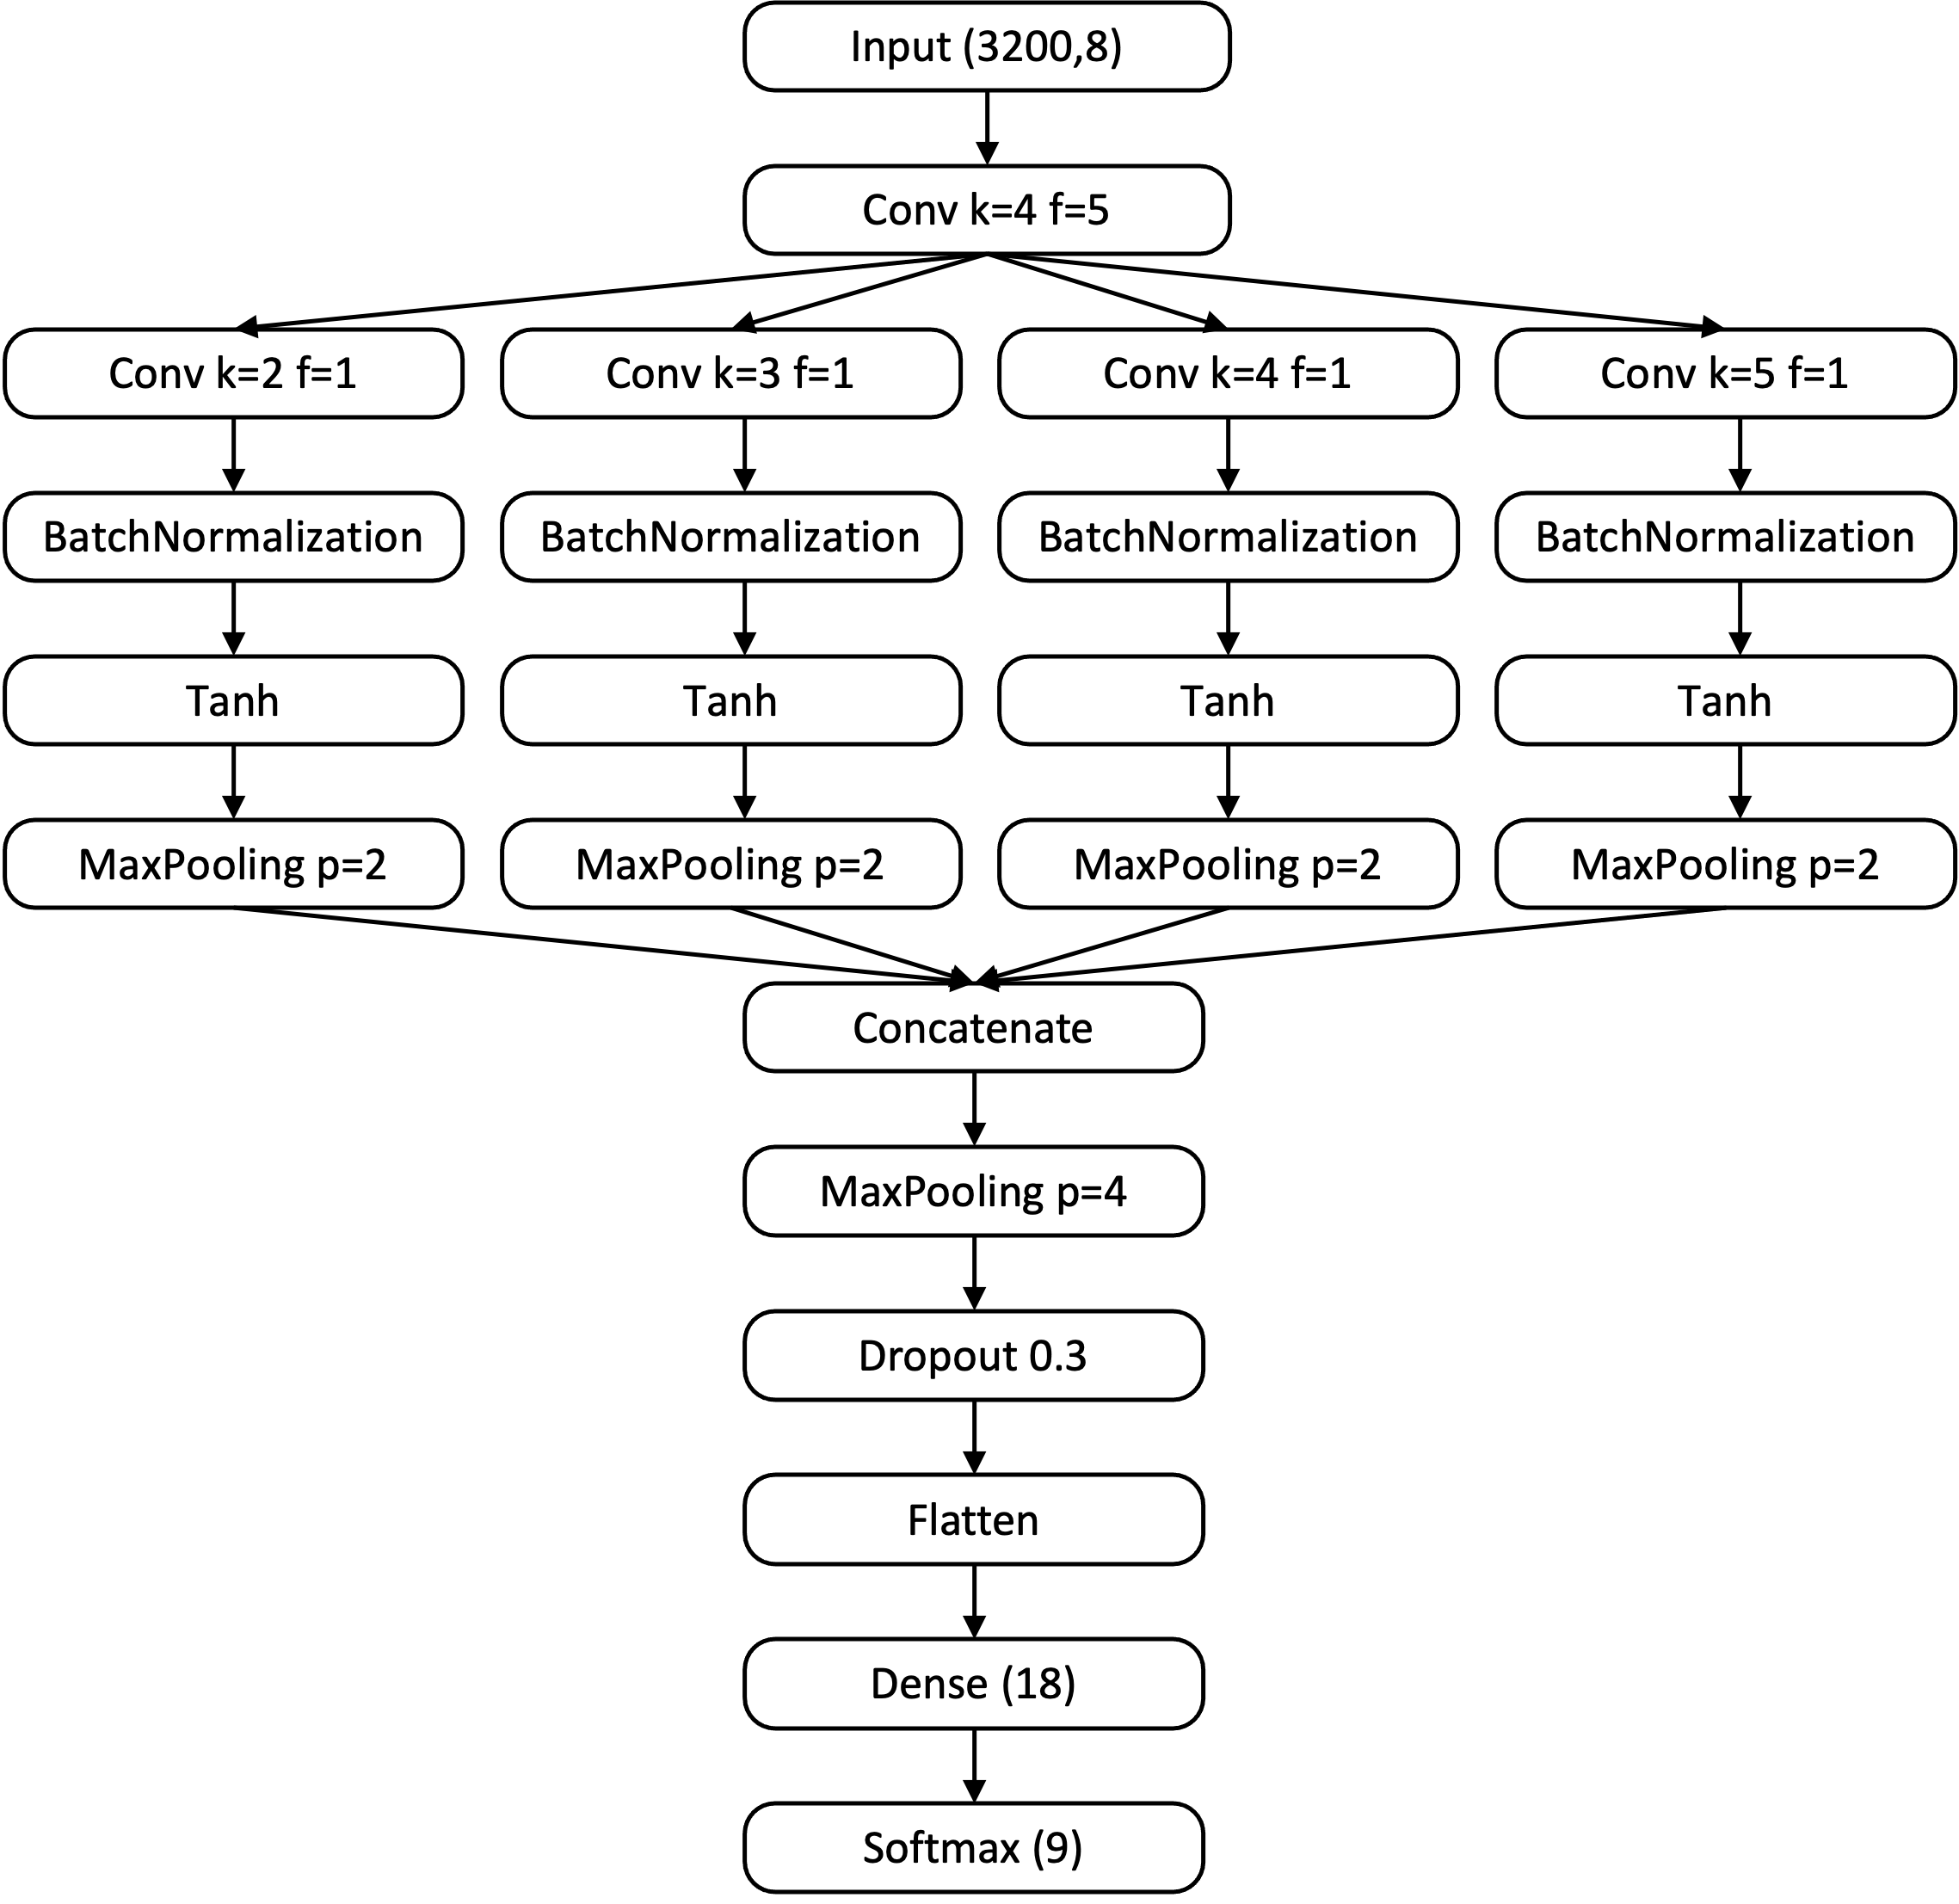
\includegraphics[scale=0.5]{img/malvecnet_model_plot.png}
    \caption{MalVecNet model plot}
    \label{fig:x MalVecNet Model Plot}
\end{figure}

\paragraph{The training}
The Hyperparameters in Table \ref{tab:x MalVecNet hyperparamters} have been used to train the MalVecNet model.
The training time was 19.4 min, and the optimum was found at epoch 76.

\begin{table}[!htbp]
    \caption{MalVecNet hyperparameters}
    \begin{center}
    \begin{tabular}{|c|c|}
    \hline 
    \textbf{\textit{Parameter}} & \textbf{\textit{Value}} \\
    \hline 
    Epochs & 100 \\
    Optimizer & Adam \\
    Learning rate & 0.0001 \\
    Loss & categorical\_crossentropy \\
    Batch Size & 40 \\
    Dense layer activation & ReLU \\
    \hline 
    \end{tabular}
    \label{tab:x MalVecNet hyperparamters}
    \end{center}
\end{table}

\subsubsection{BitNet (Byte based model)}
Lin and Yeh 2022 \cite{lin_efficient_2022} proposed a 1D representation of the byte code of the malware. 
They argued that this representation does not twist the sequential structure of the byte codes, as the fixed width of the 2D representation cuts sequential binary codes. 
The paper reports an accuracy of 0.9632\% ± 0.0078 on the BIG 2015 dataset.
\paragraph{Pre-processing}
The model uses the bytes files for classification. These files are interpreted as HEX values line by line and then converted into integers. 
All the lines are then concatenated and set to the fixed size length of 2304 using interpolation. 
After applying the interpolation, the values are again converted to integers, then converted to a binary representation, resulting in an array of 18432 integers. 
This model achieved an accuracy of 97.1\%.
During experimentation, it has also been attempted to first convert to binary, followed by interpolation. 
While this representation is not understandable to humans, very similar test accuracy has been obtained of up to 94.8\%; this configuration will be referred to as InterBitNet.

\begin{figure}[!htbp]
    \centering
    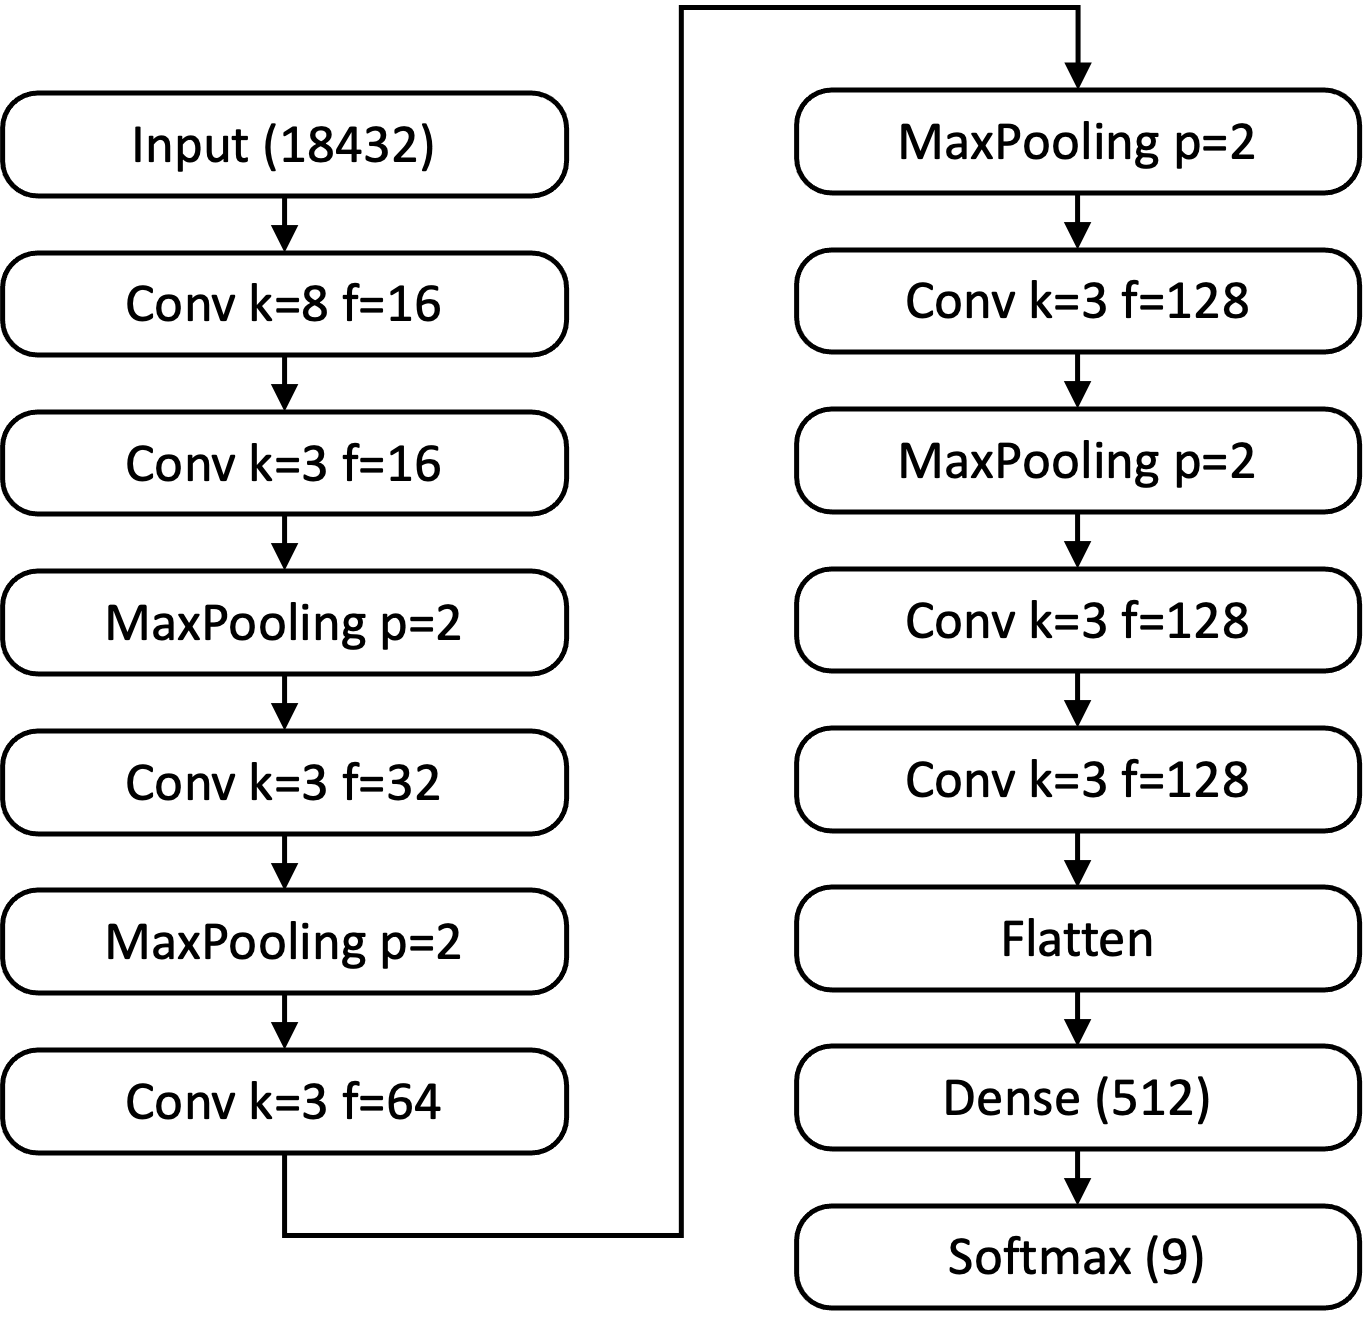
\includegraphics[scale=0.5]{img/bitnet_model_plot.png}
    \caption{BitNet model plot}
    \label{fig:x BitNet Model Plot}
\end{figure}

\paragraph{The training}
The Hyperparameters in Table \ref{tab:x BitNet hyperparamters} have been used to train the BitNet model.
The training time was 12.1 min, and the optimum was found at epoch 72.

\begin{table}[!htbp]
    \caption{BitNet hyperparameters}
    \begin{center}
    \begin{tabular}{|c|c|}
    \hline 
    \textbf{\textit{Parameter}} & \textbf{\textit{Value}} \\
    \hline 
    Epochs & 100 \\
    Optimizer & Adam \\
    Learning rate & 0.0001 \\
    Loss & categorical\_crossentropy \\
    Batch Size & 15 \\
    Alpha & 0.001 \\
    Dense layer activation & LeakyReLU \\
    \hline 
    \end{tabular}
    \label{tab:x BitNet hyperparamters}
    \end{center}
\end{table}

\subsubsection{VisNet (Entropy based model)}
The third model is based on the paper from Pinhero et al. 2021 \cite{pinhero_malware_2021}. 
They are using multiple deep learning models for malware detection and classification. 
They propose two models for malware classification, one based on VGG and one custom DNN.
\paragraph{VGG3}
The paper does not clarify how the entropy images are generated but only specifies that they are plotted with Matplotlib.
Entropy graphs shown in the paper have been recreated and used as input. 
As expected, this did not lead to good classification models as the plots incorporate many white pixels, which lack any information value.
The greyscale images used for malware detection (not classification) mentioned in the paper have been recreated and used for classification. 
However, this did not prove to be well-performing. 
Additionally, entropy images have been created in 32x32 images, which contain 1024 segments. 
The entropy values were then normalised to the scale of 0 to 255. The exact process has been used to create entropy images with the size of 256x256, which resulted in 65536 segments. 
Lastly, additional images have been created by dividing the bytes into segments of the length of 128bytes, reshaped into a squared array, and then resized. 
None of the entropy image creation methods resulted in a good classification (±75\%).
With the addition of the tremendous computational costs of this model, this has not been further pursued. 

\paragraph{DNN}
In addition to the VGG3 model for malware classification, the paper also mentioned that they used a seven-layer DNN for malware classification. They used 1282 features: 1024-block entropy values, histograms of the pixel having 256 dimensions, mean, and standard deviation.
Unfortunately, they do not describe the network architecture in detail. Over 80 different network architectures and hyperparameter settings were tested using seven fully connected layers. All models performed significantly worse than the 95\% accuracy described in the paper. 
The biggest issue was that the training was very unstable. The paper's authors have been contacted to obtain more information about the model architecture, but no response has been retrieved to this date. 
Ultimately, it has proceeded with the model with the highest accuracy of 87\%. 
OR analysis showed an accuracy of 99.48\%. 
Consequently, the model added 0.9\% of information value, despite the low accuracy.
Following this, it has been chosen to proceed with this model for the ensemble model.

\begin{figure}[!htbp]
    \centering
    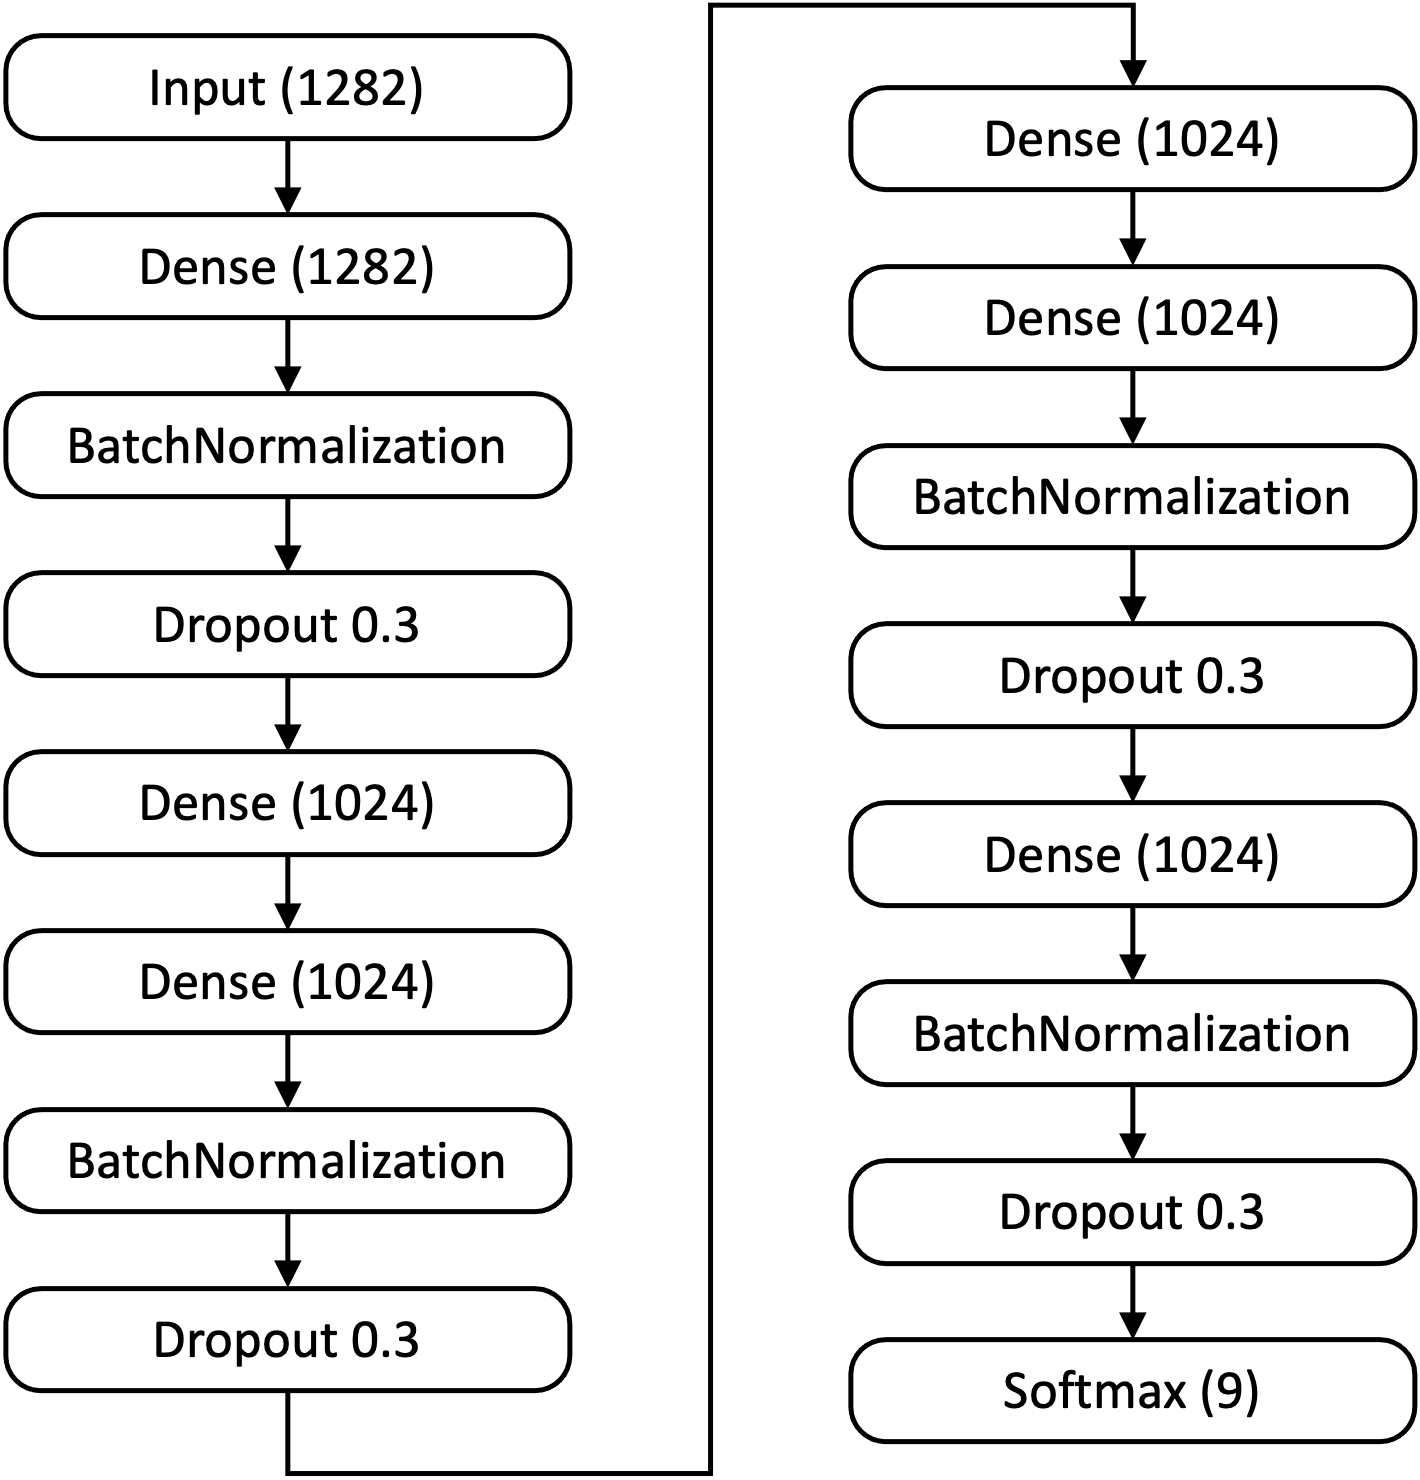
\includegraphics[scale=0.5]{img/visnet_model_plot.png}
    \caption{VisNet model plot}
    \label{fig:x VisNet Model Plot}
\end{figure}

\begin{table}[!htbp]
    \caption{VisNet hyperparameters}
    \begin{center}
    \begin{tabular}{|c|c|}
    \hline 
    \textbf{\textit{Parameter}} & \textbf{\textit{Value}} \\
    \hline 
    Epochs & 400 \\
    Optimizer & Adam \\
    Learning rate & 0.000007 \\
    Loss & categorical\_crossentropy \\
    Batch Size & 200 \\
    L1 weight decay & 0.0000001 \\
    L1 weight decay & 0.0000001 \\
    Dense layer activation & Linear \\
    \hline 
    \end{tabular}
    \label{tab:x VisNet hyperparamters}
    \end{center}
\end{table}

\subsection{Ensemble Model - EBANet}
After selecting the individual models and successfully training them, the ensemble model has been designed.
After having conducted the OR, XOR, and Top5 analysis described earlier, it was determined that the optimal accuracy obtainable with the pre-trained models is 99.44\%. 
A multitude of designs has been created and tested, and each one of them reached an accuracy of at least 98\%.
The model proposed in this dissertation will be called Entropy, Bytes and Assembly input Network (EBANet).

\paragraph{The architecture}
With this in mind, two designs should be outlined. 
The first is worthy of being mentioned due to its simplicity. 
It only features a concatenation of all the outputs from the individual models, followed by a hidden layer using 27 neurons and ReLU as activation function and a fully connected output layer featuring nine neurons using softmax.
Using this simple design, an accuracy of 98.3\% could be reached. In this configuration, only the dense layers for the ensemble are trainable. 
The individual models are frozen.
While this has not been further investigated for reasons explained in chapter \ref{eager}, initial results suggest that this simple model could be improved solely by training it using the graph mode.

The first configuration is very simple and quick to train, as the individual models are pre-trained, and only 1008 parameters must be trained. 
However, this will not result in the best performance possible, as the models have not been trained to work together.
Through experimentation, it has been found that the best performance can be achieved by pre-training the individual models and then freezing them. The ensemble connection is then trained, and the entire ensemble is trained together by unfreezing the individual models and using auxiliary outputs.
On top of this, the ensemble has been made more complex. 
Throughout experiments, it has been found that combining just two models of the three will result in a combined performance of 97-98\%.
Therefore, a more complex model has been designed, which used additional layers and combined the models in different ways to get the best performance possible.
This design is based on ensemble models built during this project which combine two individual models into an ensemble.
The model plot can be seen in Figure \ref{fig:x emp}. This architecture reached a test accuracy of 98.7\%.

\begin{figure}[!htbp]
    \centering
    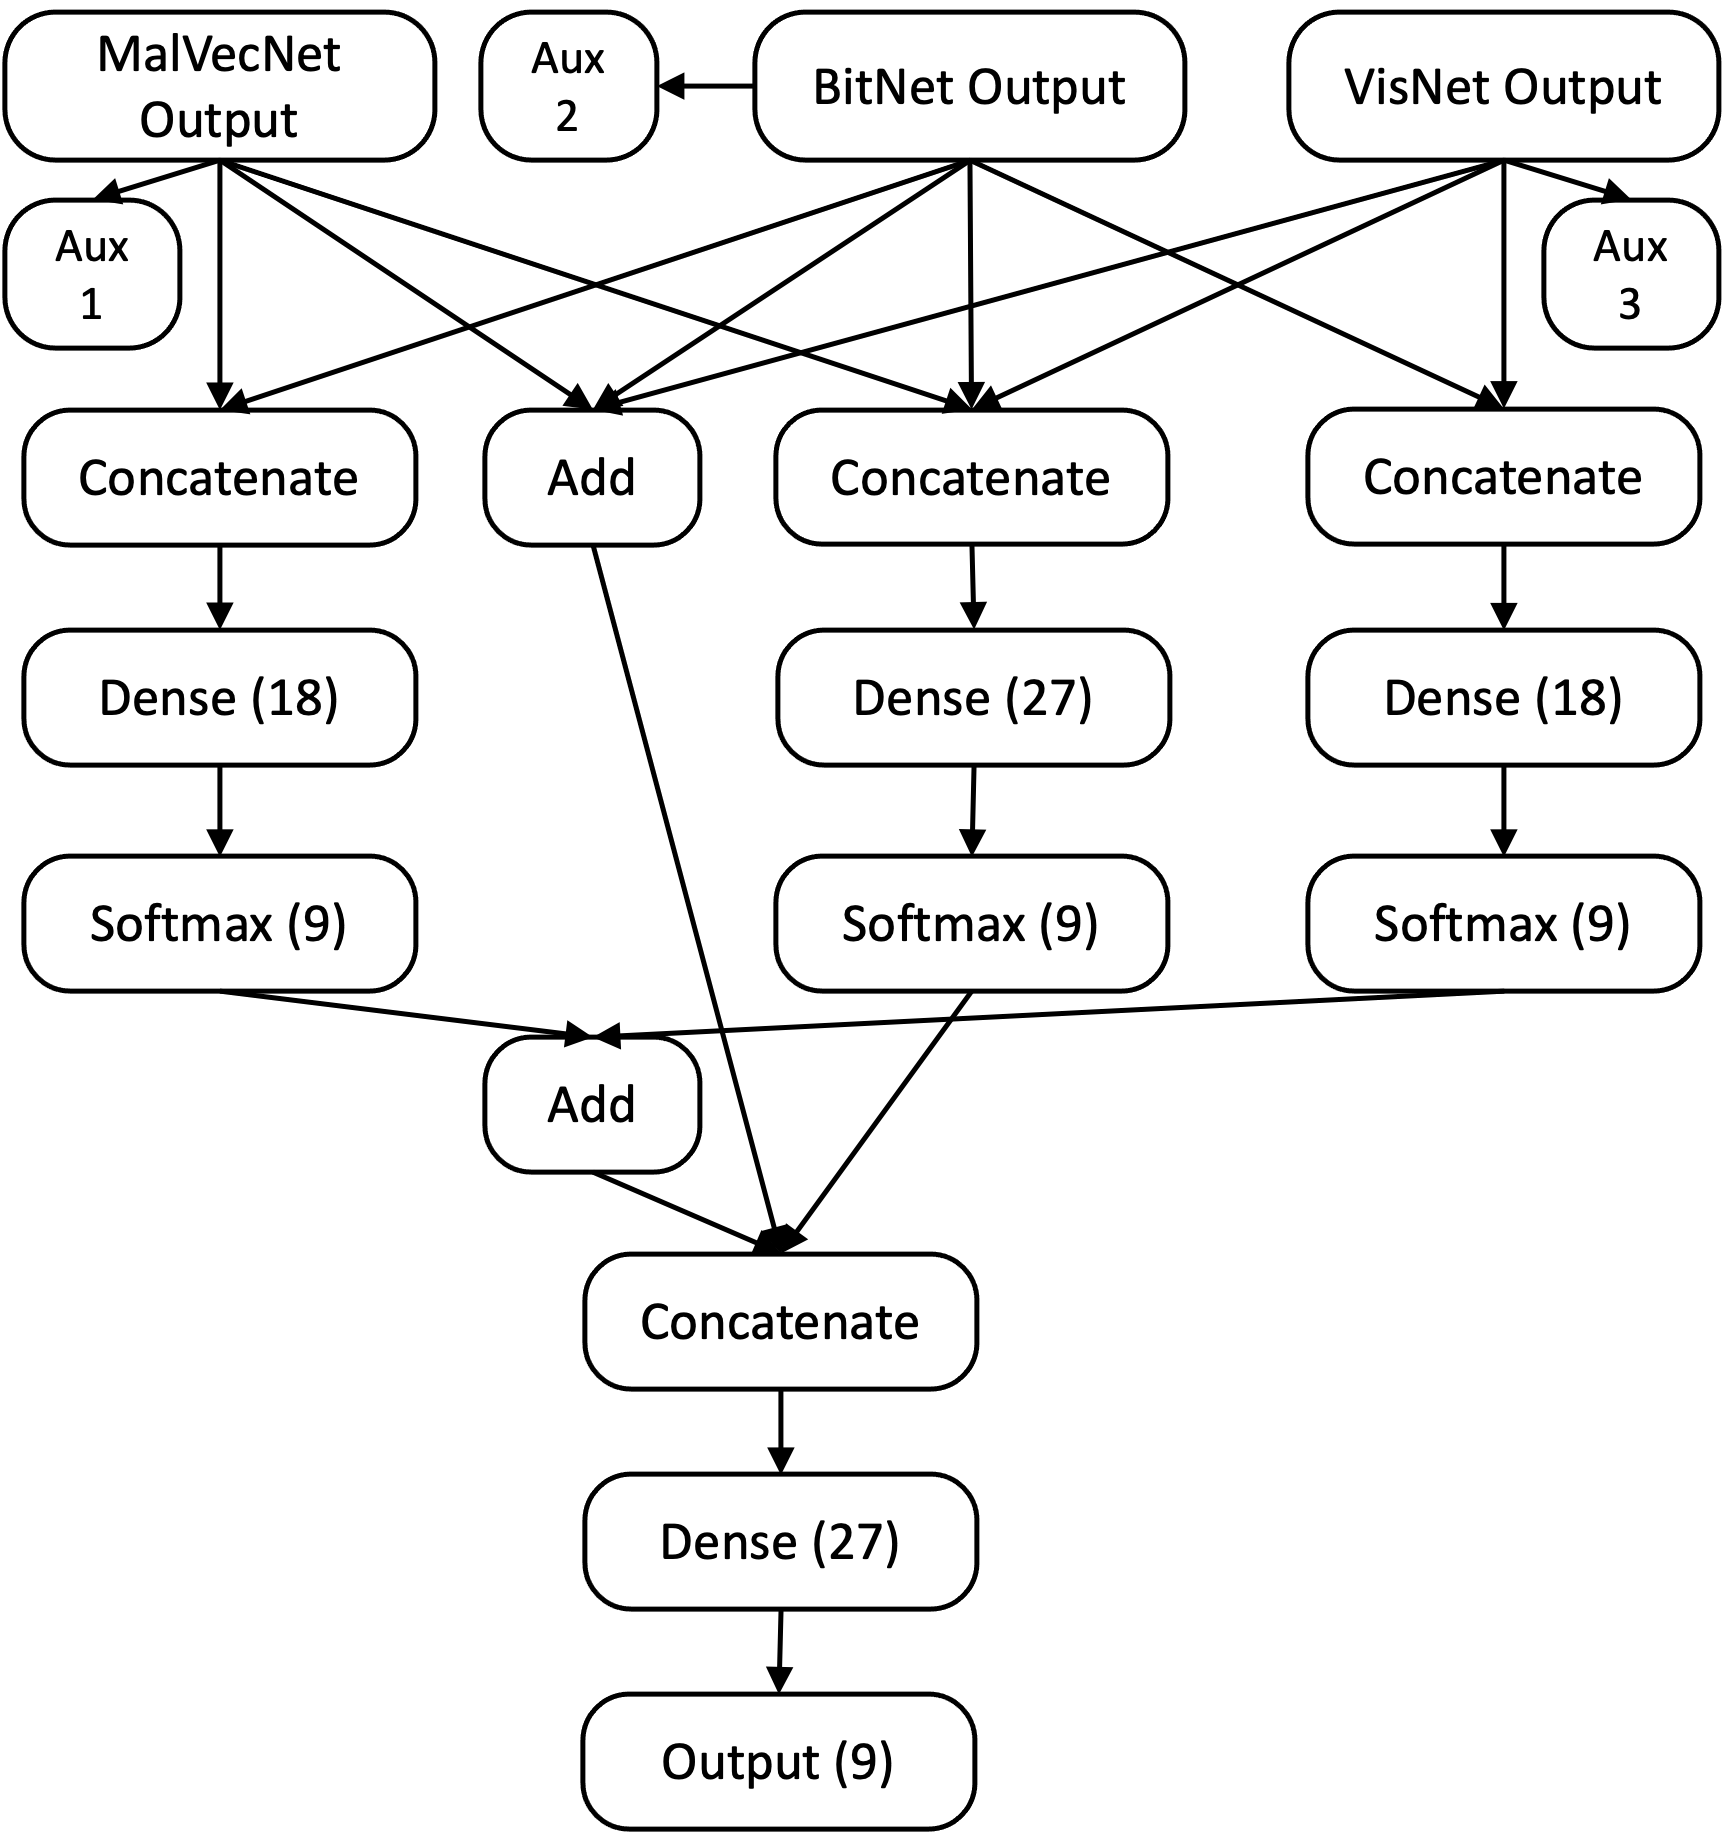
\includegraphics[scale=0.4]{img/ensemble_model_plot.png}
    \caption{EBANet Model Plot}
    \label{fig:x emp}
\end{figure}

\begin{table}[!htbp]
    \caption{EBANet model hyperparameters}
    \begin{center}
    \begin{tabular}{|c|c|}
    \hline 
    \textbf{\textit{Parameter}} & \textbf{\textit{Value}} \\
    \hline 
    Epochs (first phase) & 100 \\
    Epochs (second phase) & 100 \\
    Optimizer & Adam \\
    Learning rate & 0.0001 \\
    Loss & categorical\_crossentropy \\
    Batch Size & 30 \\
    Dense layer activation & ReLU \\
    \hline 
    \end{tabular}
    \label{tab:x Ensemble hyperparamters}
    \end{center}
\end{table}

\subsection{The Enviroment}
All experiments presented in this paper have been performed using the setup explained in this chapter. 
In addition, version control has been achieved using git and GitHub.
\subsubsection{Runtime}
The experiments were conducted within a Google Colab-Pro environment using a T4 GPU with the Keras framework. 
The code and dataset have been stored on Google Drive. 
Before every run, the pre-processed dataset was copied into the Colab environment, so the limited bandwidth between Google Drive and Google Colab would not impact the training time.
In its final version, the code has been adapted to run without Google Colab on a local machine and to be self-sustained within the Git repository to improve reproducibility.
\subsubsection{MLflow}
\paragraph{Tracked Parameters}
For each run, between 12 and 25 parameters, 12 metrics and six artefacts have been stored. 
This included a version of the python script for easy reproducibility.
\paragraph{Colab Setup}\label{colab}
For experiment logging, mlflow has been used. 
Initial experiments have been logged on a local mlflow server running on Google Colab using Ngrok. 
Due to resource limitations given by Colab, this setup reached its limits after 110 runs.
\paragraph{Databricks Setup}
As the Colab Setup quickly reached its limits, the Databricks Community version of mlflow has been used temporarily. 
The Databricks servers provided excellent performance, but this setup led to data loss, as the account used was blocked due to unusual activity caused by the connection coming from the Google Colab server, which was classified as bot behaviour.
\paragraph{Docker Setup}
As both the Databricks Community Server and the mlflow server running on Colab did not provide the stability required for this project, a personal mlflow server has been deployed using Docker, Ngrok, Minio, MySQL \& mlflow. 
All components required have been containerised and deployed on a MacBook. 
Using Ngrok, two tunnels using HTTP authentication, one to the Minio S3 storage and one to the mlflow server, have been opened. 
These tunnels allowed the Google Colab server to communicate with the mlflow server and the Minio S3 storage for artefact storage.
\paragraph{Summary}
Ultimately, the Docker configuration proved to be very reliable.
Nevertheless, this outlines that the field of ML/AI is in its early stages, as tools for version control, logging, tracking, and testing are widely available and easily accessible for other fields of computer science but not for AI.
While mlflow proved to be a very effective tool, the configuration requires much effort and expertise. 
Moreover, tools such as Apache Spark, which could make the data pipeline more structured and allow easy version control, require even more effort to be configured. 
To achieve better reproducibility of work in the AI/ML field, these tools need to be made more accessible.

\paragraph{The training}\label{ensemble_training}
The following Hyperparameters in Table \ref{tab:x Simple ensemble hyperparamters} have been used to train the simple ensemble. 
The model with the lowest loss has been used for testing, which occurred at epoch 152.

\begin{table}[!htbp]
    \caption{Simple ensemble model hyperparameters}
    \begin{center}
    \begin{tabular}{|c|c|}
    \hline 
    \textbf{\textit{Parameter}} & \textbf{\textit{Value}} \\
    \hline 
    Epochs & 200 \\
    Optimizer & Adam \\
    Learning rate & 0.0001 \\
    Loss & categorical\_crossentropy \\
    Batch Size & 30 \\
    Dense layer activation & ReLU \\
    \hline 
    \end{tabular}
    \label{tab:x Simple ensemble hyperparamters}
    \end{center}
\end{table}

The training has been split into two phases for the more complex model.
In the first phase, only the layers for the ensemble are trained, while the layers from the individual models are frozen.
After the first phase, the model with the lowest loss will be loaded for the second phase.
In the second phase, all layers are trainable. 
This allows the individual models to adjust to each other, and by them learning to work together, the overall result increases.
The second phase performs slightly better when using auxiliary outputs, as this ensures that, while training, the overall performance and the performance of the individual models are monitored.
The detailed hyperparameter can be found in Table \ref{tab:x Ensemble hyperparamters}. 
Unfortunately, using auxiliary outputs comes with the cost of not being able to define class weights, which is another issue of the Tensorflow framework. 
The related GitHub issue is: https://github.com/tensorflow/tensorflow/issues/41448 \cite{noauthor_tfkeras_nodate}. 
Therefore, using auxiliary outputs does increase the accuracy but does not decrease the performance of minority classes. This can be seen when comparing Figure \ref{fig:a ensemble model Confusion Matrix with auxiliary output} and \ref{fig:a ensemble model confusion matrix without auxiliary output}. 
Both models have the same architecture and training procedure, but the model without auxiliary outputs uses class weights.


\paragraph{Eager Execution}\label{eager}
Since Tensorflow 2.0, eager execution has been the standard method, generally preferred over graph execution. 
This goes to the extent that some layers nowadays cannot even be executed using the graph anymore. 
One example is the BatchNormalization layer. 
This has been discovered during experimentation. 
Having witnessed better results when training the Ensemble model in graph mode, an attempt to train the other models that utilise BatchNormalization layers into graph mode has also been made. 
However, this resulted in an error. This behaviour cannot yet be explained, but it has ultimately been found to relate to this GitHub issue: https://github.com/tensorflow/tensorflow/issues/35107 \cite{noauthor_tfkeraslayersbatchnormalization_nodate}. 
For this reason, the testing within this paper is limited to the individual models being trained eagerly.

\section{Results}\label{C4}

In this chapter, the results of the individual models, as well the results of the ensemble model, will be presented and discussed. 

\subsection{MalVecNet}
As previously mentioned, this model has been altered after detecting a data leakage mistake in the original paper.
Despite this, the original model has been trained and tested, using the same data preprocessing as the original paper an accuracy of 97.8\% was achieved. 
Without data leakage, the model accuracy dropped below 67\%.
After having modified the model as described in chapter \ref{malvecnet}, an accuracy of 90.5\% could be achieved.

The model mainly struggled with classes 4,5 and 7 (see Figure \ref{fig:a malvecnet Confusion Matrix}); this is in accordance with the original paper. 
This suggests that these classes are more difficult to detect when analysing disassembled code.

\subsection{BitNet}

The results of BitNet are in line with the results presented in the original paper. 
Surprisingly, the replicated model did perform slightly better, as the paper reported an accuracy of 96.32\% and the replication achieved an accuracy of 97.05\%.
It has been mentioned that InterBitNet has been trained with a different preprocessing method, which only achieved an accuracy of 95\%. 
Using BitNet or InterBitNet did not change the results of the ensemble model significantly. 
Using BitNet only improved the ensemble model accuracy by 0.1\%, although it is 2\% better than InterBitNet.

\subsection{VisNet}

VisNet was the worst-performing model of the three, with an accuracy of 87.6\%.
The training was highly unstable, with the validation accuracy strongly fluctuating (see Figure \ref{fig:b VisNet training plot}).
This behaviour could not be improved by using weight-decay, altering learning rates, dropouts, verity of normalisations and activation functions.
Using different model designs was not preventing the fluctuation either. This model should be replaced by a different entropy model in the future.
However, as mentioned earlier, the model adds information value to the ensemble despite the inadequate training.


\subsection{EBANet}
EBANet does not reach the theoretical optimum of 99.42\% calculated using the or analysis. 
With 98.7\% it represents a significant improvement of the individual models.
EBANet only finds two new samples that none of the individual models found.
This showcases that training the ensemble together, with all layers trainable, did not lead to the individual models finding new samples but only helped the models to work better together.

\begin{table}[!htbp]
    \caption{Results}
    \begin{center}
    \begin{tabular}{|c|c|c|c|c|}
    \hline 
    \textbf{\textit{Model}} &\textbf{\textit{Accuracy}} & \textbf{\textit{Loss}}& \textbf{\textit{Recall}}& \textbf{\textit{Precision}} \\
    \hline 
    \textbf{MalVecNet} & 90.5\% & 0.375\%  & 89.4\%  & 92\% \\
    \textbf{BitNet} & 97.1\%  & 0.117\% & 97\% & 97.5\% \\
    \textbf{VisNet} & 87.6\% & 0.45  & 82.2\%  & 91.1\% \\
    \hline
    \textbf{EBANet} & 98.7\% & 1.654 & 96.7\% & 96.8\% \\
    \hline 
    \end{tabular}
    \label{tab:x Results}
    \end{center}
\end{table}

\subsection{Results Analysis}
After having trained the individual models, the predictions have been analysed and compared, as described in chapter \ref{analysis}. 
Figure \ref{fig:x model_accuracy_chart} shows the models' results compared to the OR and the AND analysis.
This outlines that while the models over the OR have very high accuracy, the models do have a very low overlap of only 80.58\%.
In figure \ref{fig:x unique_preditctions_normal} the number of unique predictions for each model in each malware class is visualised. 
The graph outlines that each model has focused on specific malware classes and that the three models complement each other. 
It should be mentioned that while this graph is an excellent visual aid, it does not portray the whole truth. 
Each model did not specialise in detecting specific malware classes; instead, they specialised in detecting certain ways of malware structures, programming techniques and obfuscation methods.
These correlate but only have indirect causation with the malware classes, which is why this graph can be used as a visual aid to outline the specifications of the models without having to conduct a deep malware analysis on each predicted sample.

\begin{figure}[!htbp]
    \centering
    \begin{subfigure}[b]{0.24\textwidth}
        \centering
        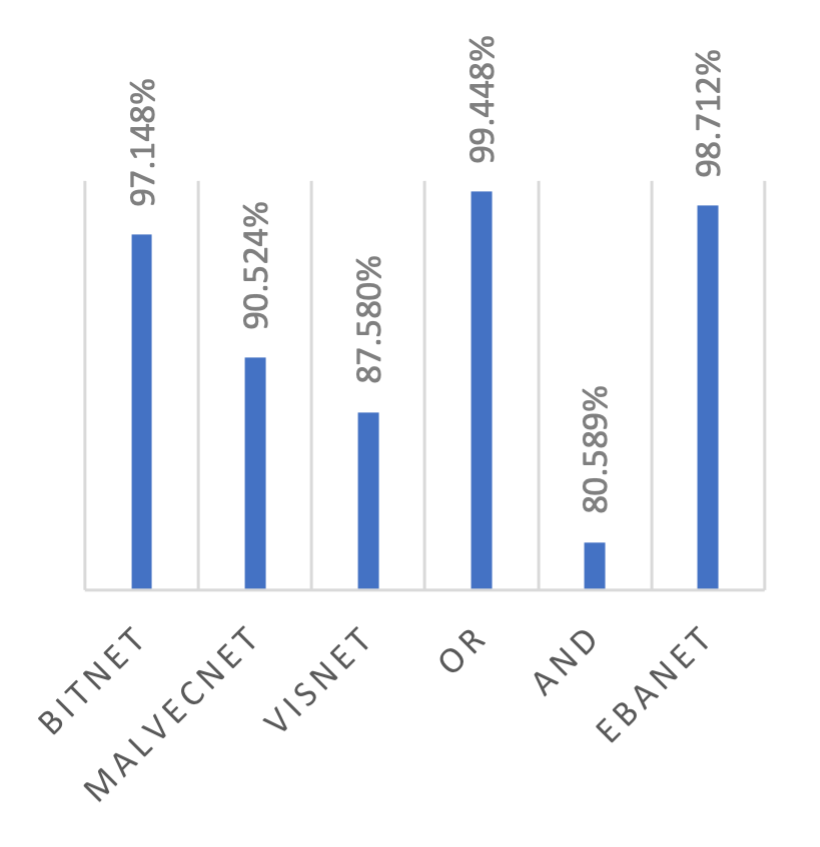
\includegraphics[scale=0.65]{img/model_accuracy_chart_small.png}
        \caption{Model accuracies and comparison and prediction}
        \label{fig:x model_accuracy_chart}
    \end{subfigure}
    \hfill
    \begin{subfigure}[b]{0.24\textwidth}
        \centering
        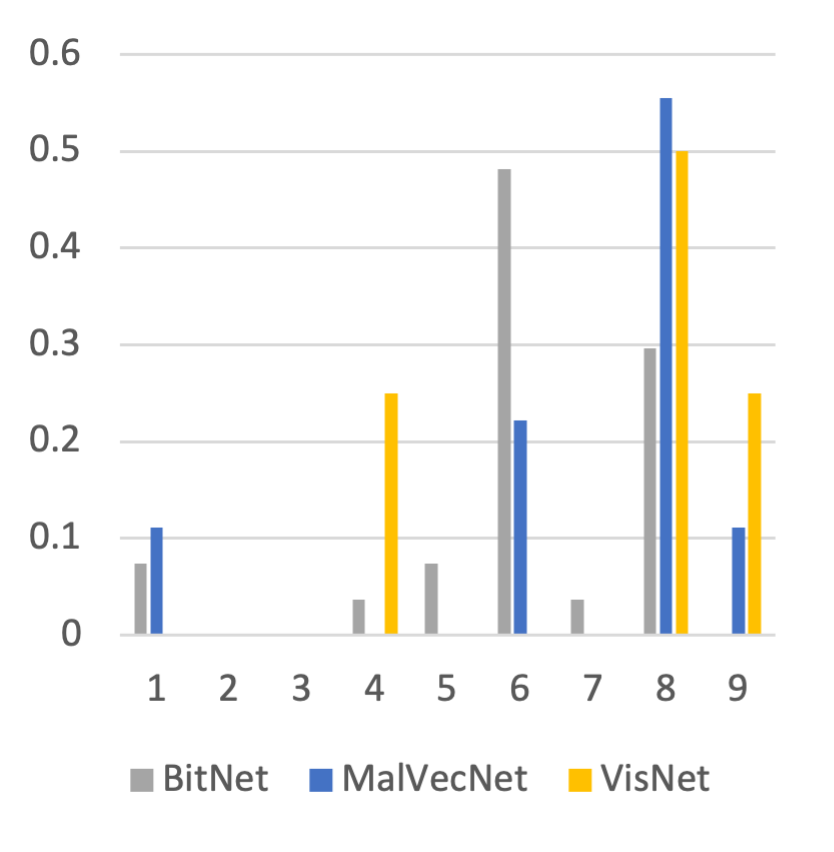
\includegraphics[scale=0.65]{img/unique_preditctions_normal_small.png}
        \caption{Unique predictions of each model by class (normalised)}
        \label{fig:x unique_preditctions_normal}
    \end{subfigure}
    \caption{Analysis Plots}
    \label{fig: Analysis Plots}
\end{figure}

Together the graphs in Figure \ref{fig:x model_accuracy_chart} \& \ref{fig:x unique_preditctions_normal} show that not only the accuracy improves by using the ensemble, but the models complement each other by detecting different samples based on their specialisation defined by their input/preprocessing, similar to how malware analysts detect differently attributes during different analyses.

\subsection{Leasons Learned}
The observations made while analysing all runs captured using mlflow are outlined in this section. 

The most significant observation made during the experiments for MalVecNet was that increasing batch size instead of decaying learning rate worked significantly better. This was inspired by the paper 'Don't Decay the Learning Rate, Increase the Batch Size' by Smith et al. 2018 \cite{smith_dont_2018}.

While experimenting with VisNet, in an attempt to understand the behaviour of the model, the model has been trained on a leaky dataset. 
Against expectations, this did not improve the validation accuracy of the model. 
The effect was the opposite. 
This showed that the fluctuating behaviour did not derive from the model overfitting onto a local optimum.
While highly unusual, this test was very successful in this specific scenario.

For all models, it could be observed that using SGD instead of Adam did not impact the model's outcome, but the learning rate for SGD had to be increased by a factor of 10$^3$ compared to Adam.

The last significant observation made is regarding the minority classes. 
Throughout this dissertation, two methods have been used to balance the learning for all classes. 
One method was upsampling the training dataset, and the other was to use class weights. For all models, both methods improved the accuracy of minority classes.
Nevertheless, only for MalVecNet using Upsampling improved the overall accuracy. All other models did suffer from lower accuracy over all classes when using upsampling. This was also true for EBANet, where class-weights could not be used due to the auxiliary outputs (\ref{ensemble_training}).

\section{Discussion}\label{C5}

\subsection{Why Open Source is important}
Errors in papers like Jiang et al. 2019 represent why reproducibility is essential. 
Additionally, even in the peer review process, sometimes mistakes happen. 
The author of this dissertation wants to use these lines to outline the importance of publishing the source code of ML models so that results can be reproduced and verified. 
Moreover, this allows for a more exhaustive comparison of models. 
In addition, if the code is shared, future researchers can use previous models in their testing environment, which allows for a direct comparison of results and a more concrete outline of improvements over previous works.

\subsection{Discussion of Results}
The project has been completed successfully, as it has been possible to prove the original theory that using multiple representations of malware can improve performance, as different representations will allow for the detection of different malware.
On top of that, the results of this project have shown that using an ensemble of multiple low-performing models, which all focus on specific classes of samples, can lead to a high-performance ensemble model. 
While the model is not breaking any records in performance, the results are in line with current models and outperform some of them while being less complex than most of them. 
This can be attributed to the fact that this model uses the methodology of malware analysts as a basis for its design.
This shows that AI research can highly benefit from using concepts and approaches from the existing fields and developing models that mimic them instead of trying to find new approaches.

Nevertheless, this project did have some shortcomings that limited the outcome. 
One great limitation was that two of the three replicated models did not describe the model architecture enough in detail to replicate them, leading to the replicated models performing poorly as a consequence, even after extended experimentation.

Although the focus of this project was a proof of concept, the final accuracy of EBANet should be discussed. 
The final EBANet model achieved an accuracy of 98.7\%. 
Papers released within the last two years using the Microsoft BIG 2015 dataset have achieved an accuracy from 93.19\% up to 98.74\% (\cite{lin_efficient_2022},\cite{pinhero_malware_2021},\cite{hemalatha_efficient_2021},\cite{kumar_dtmic_2022},\cite{kwon_malware_2020},\cite{sun_categorizing_2020}), leaving the results of this paper at the upper end of current proposals.

\section{Future work}\label{C6}
While this paper lays the ground idea for creating malware classification models based on multiple malware representations, the individual models could be improved in future work. 
VisNet did perform very poorly and could be replaced with a model that performs better using entropy inputs. 
On top, more models could be added to the ensemble, incorporating more representations, thereby improving the model. 
Smith et al. 2017 \cite{smith_mind_2017} have argued that adding dynamic information would close the gap to the field of MA even further.

Despite improving the model, the model deployment issue needs to be addressed in the future. 
To the best of the author's knowledge, currently, no open-source automated data pipeline can be used to input the executable and output the disassembled code so that a model like this could be deployed and used in production.

Lastly, the concept presented in this paper could be used on tasks such as malware detection. 
Previous papers such as Pinhero et al. \cite{pinhero_malware_2021} show that models designed for classification or detection could potentially be used interchangeably.
It is the author's belief that the multi-representation methodology of this model would allow for better detection in the long term.

\printbibliography

\clearpage
\appendix
\counterwithin{figure}{section}
\setcounter{figure}{0}
\subsection{Confusion Matrixes}\label{appendix:matrixes}
\counterwithin{figure}{subsection}

\begin{figure}[H]
    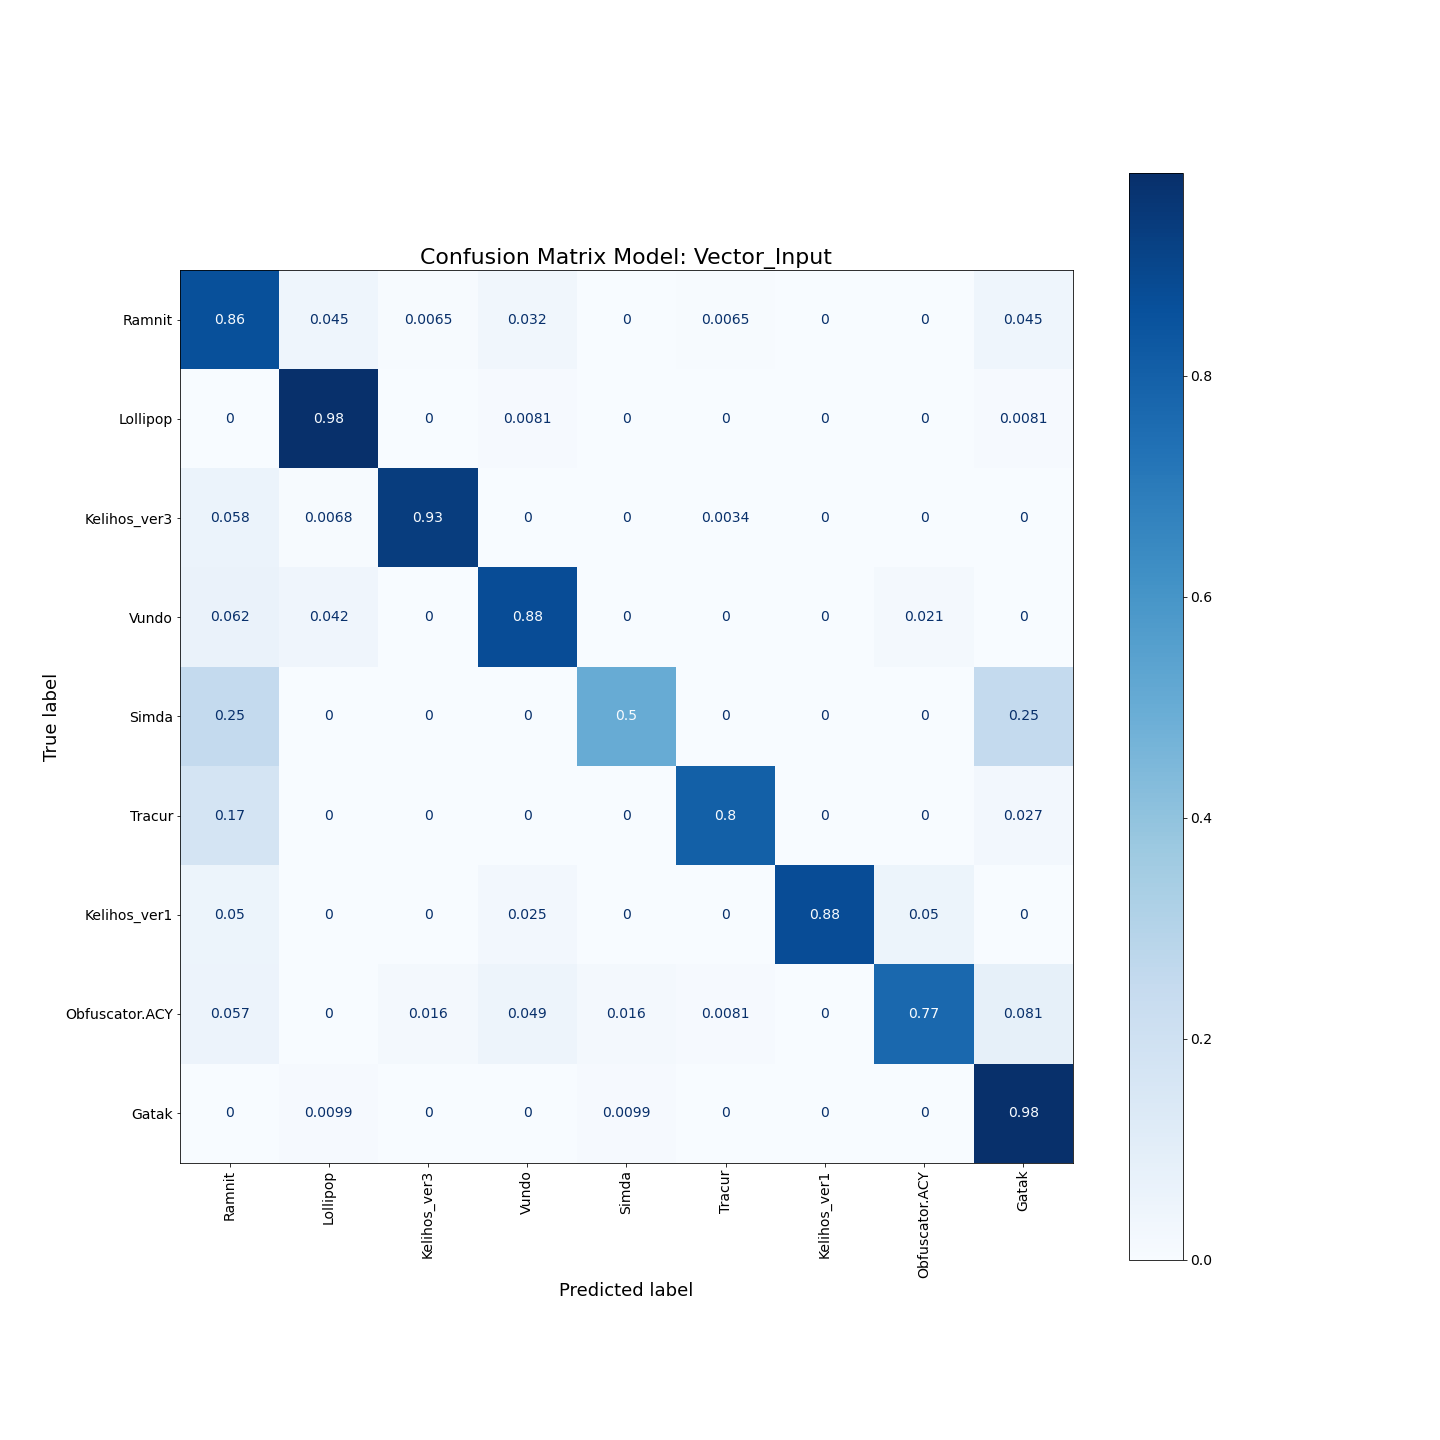
\includegraphics[scale=0.19]{img/malvecnet_confusion_matrix.png}
    \caption{MalVecNet confusion matrix}
    \label{fig:a malvecnet Confusion Matrix}
\end{figure}
\begin{figure}[H]
    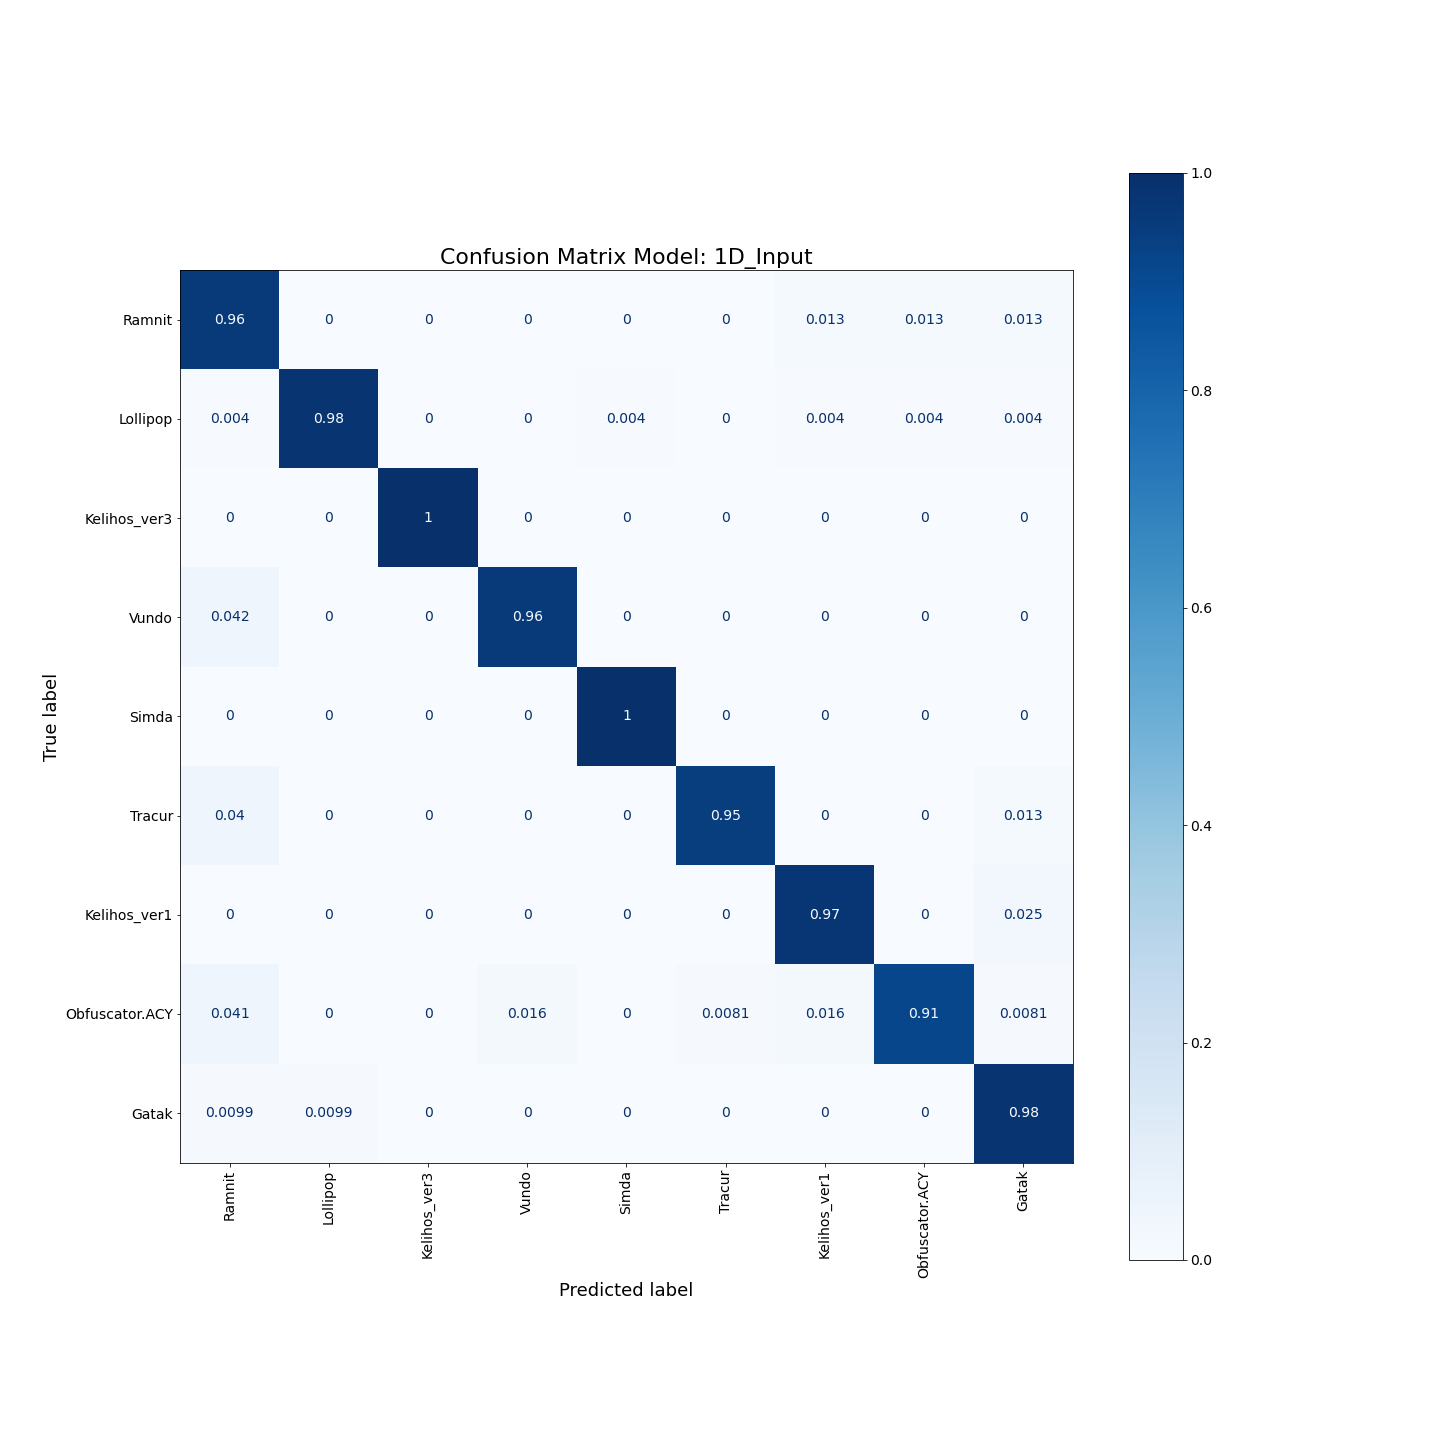
\includegraphics[scale=0.19]{img/bitnet_confusion_matrix.png}
    \caption{BitNet confusion matrix}
    \label{fig:a BitNet Confusion Matrix}
\end{figure}
\begin{figure}[H]
    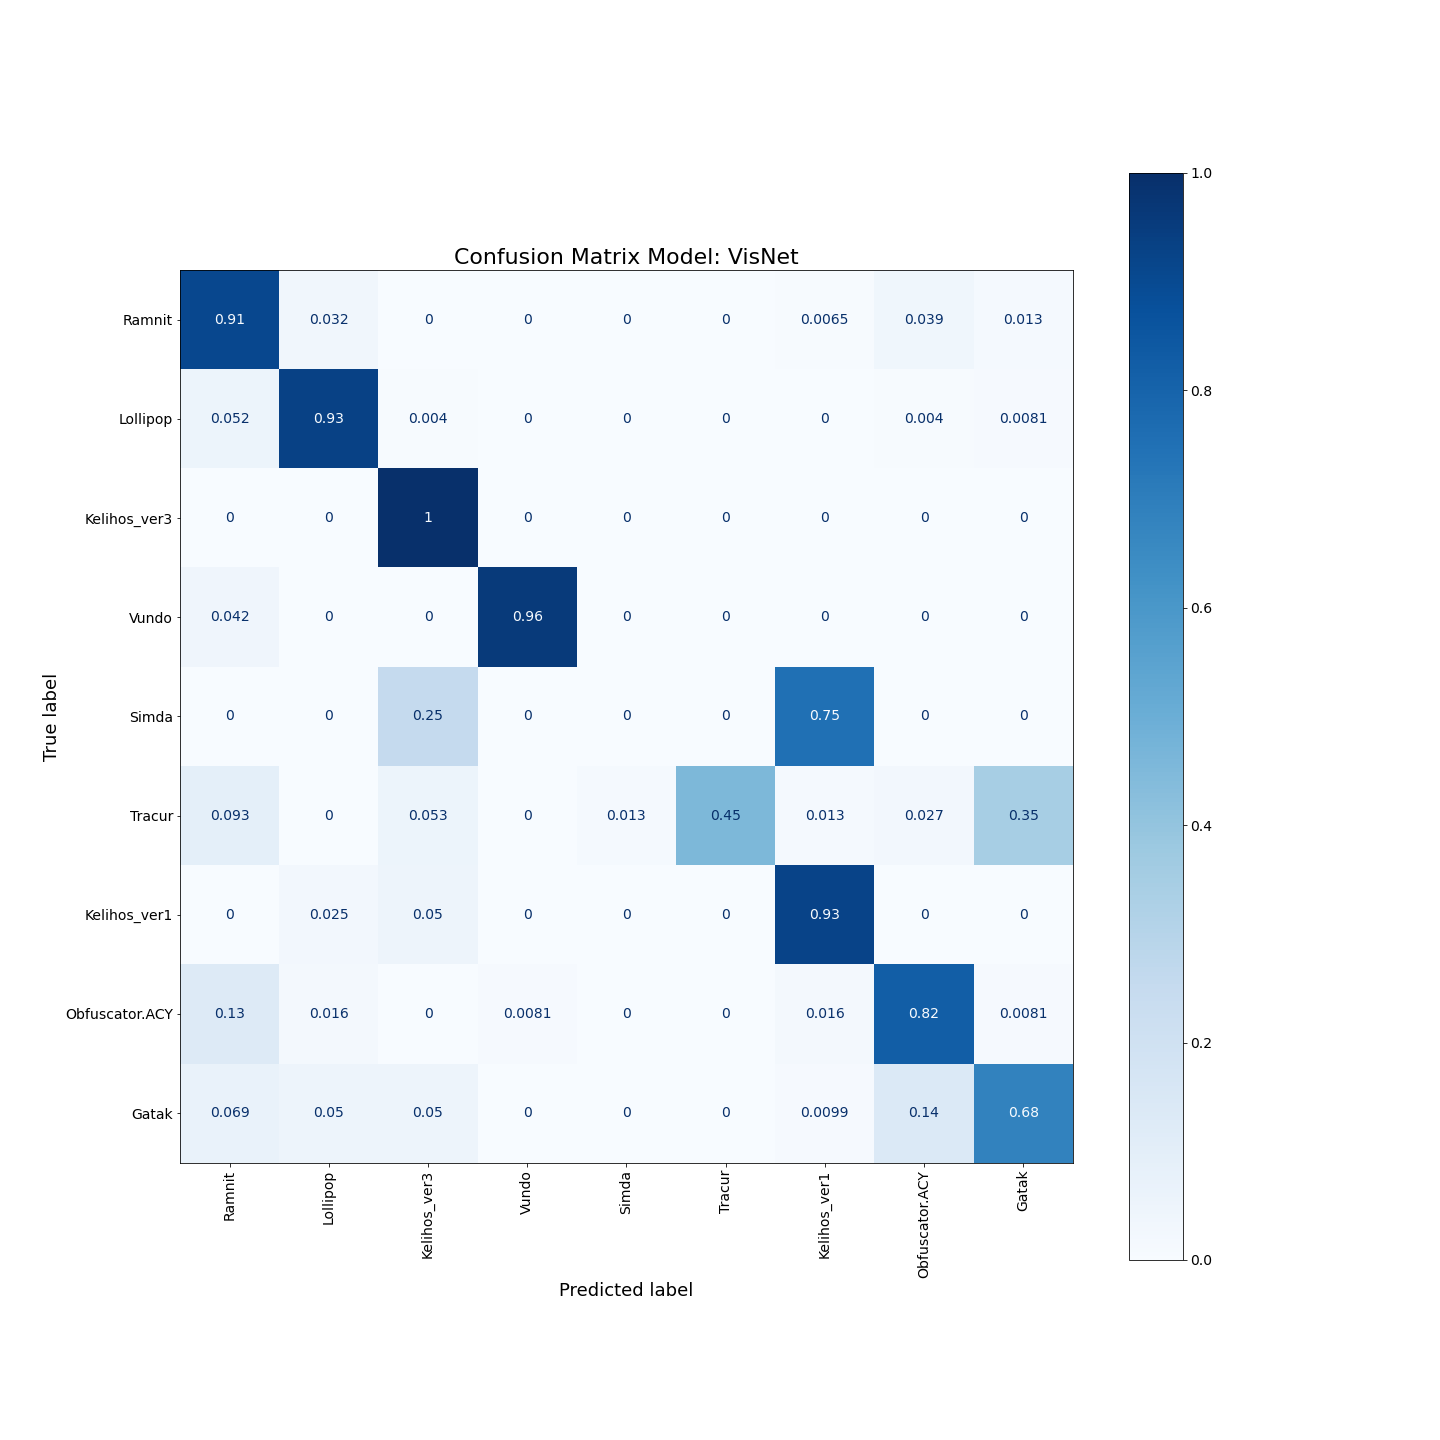
\includegraphics[scale=0.19]{img/visnet_confusion_matrix.png}
    \caption{VisNet confusion matrix}
    \label{fig:a VisNet Confusion Matrix}
\end{figure}
\begin{figure}[H]
    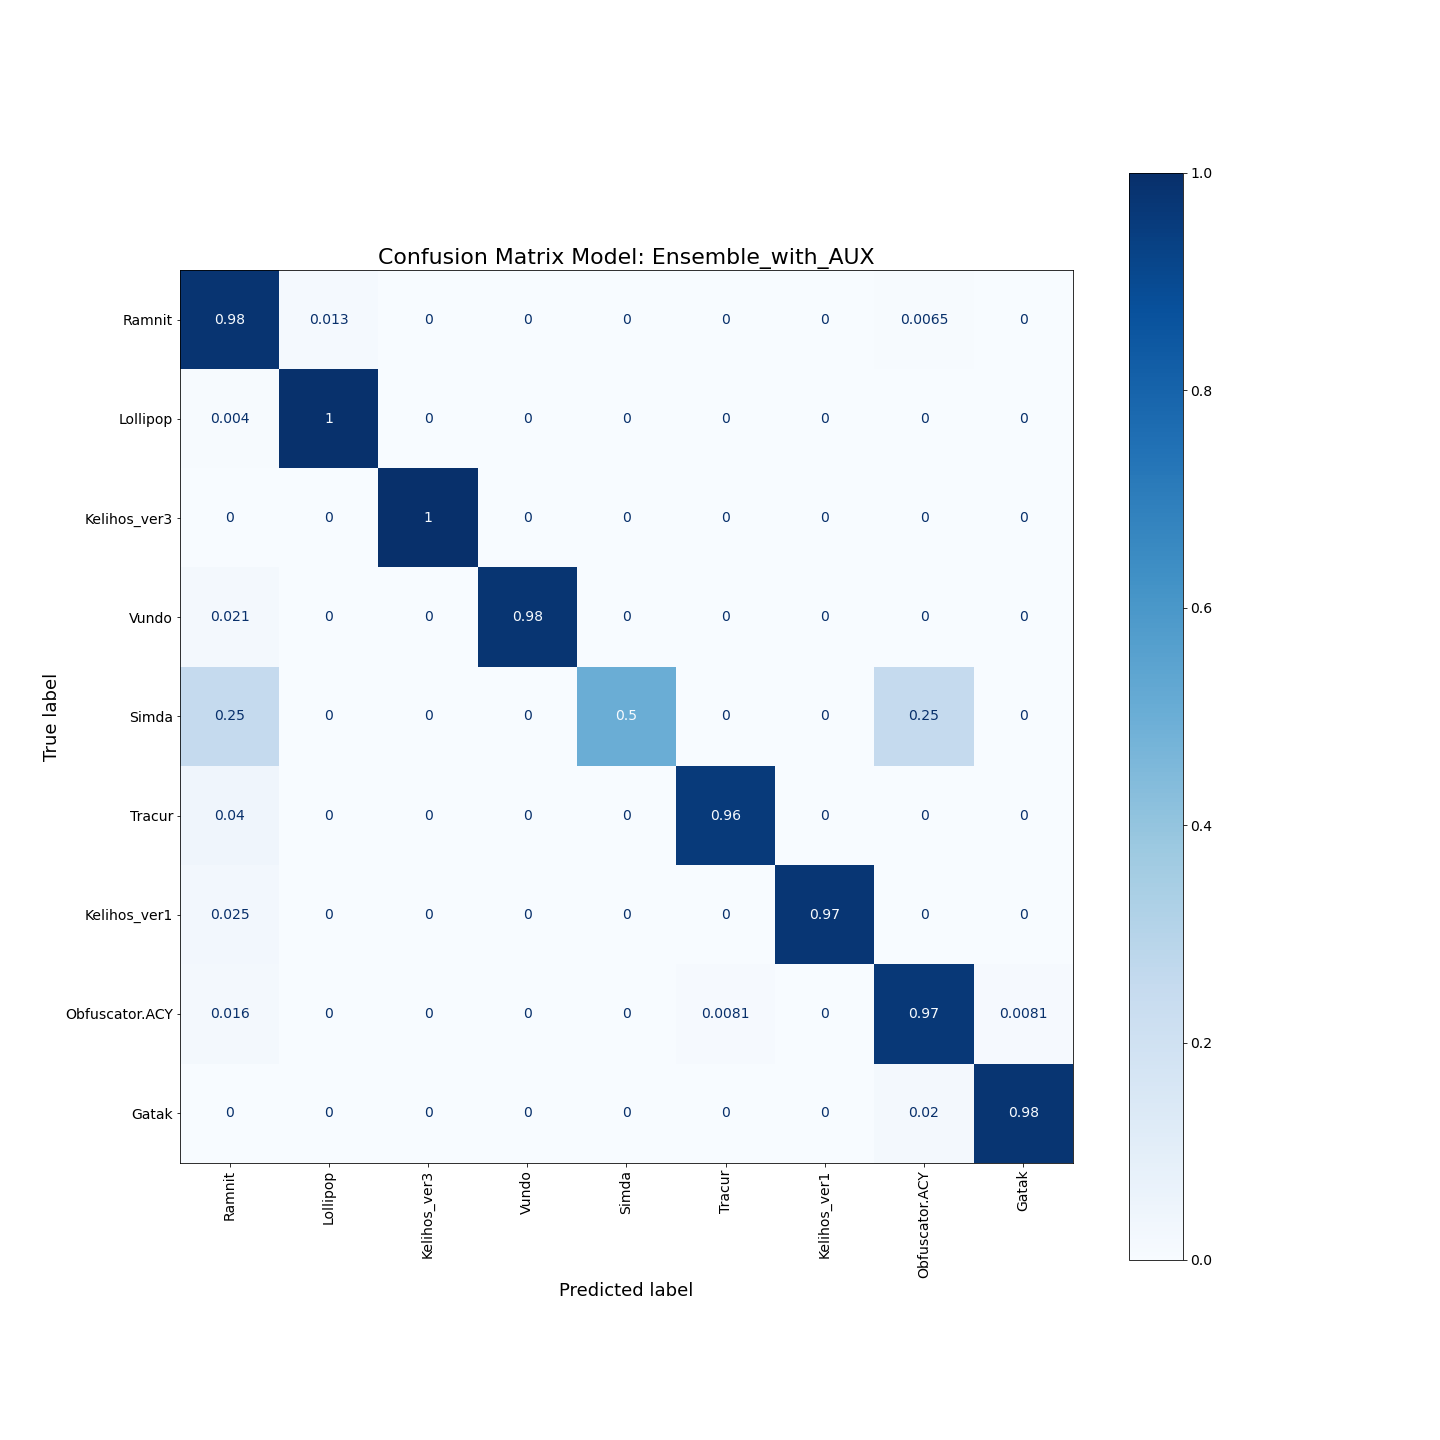
\includegraphics[scale=0.19]{img/confusion_matrix_aux_4.png}
    \caption{EBANet confusion matrix with auxiliary output}
    \label{fig:a ensemble model Confusion Matrix with auxiliary output}
\end{figure}
\begin{figure}[H]
    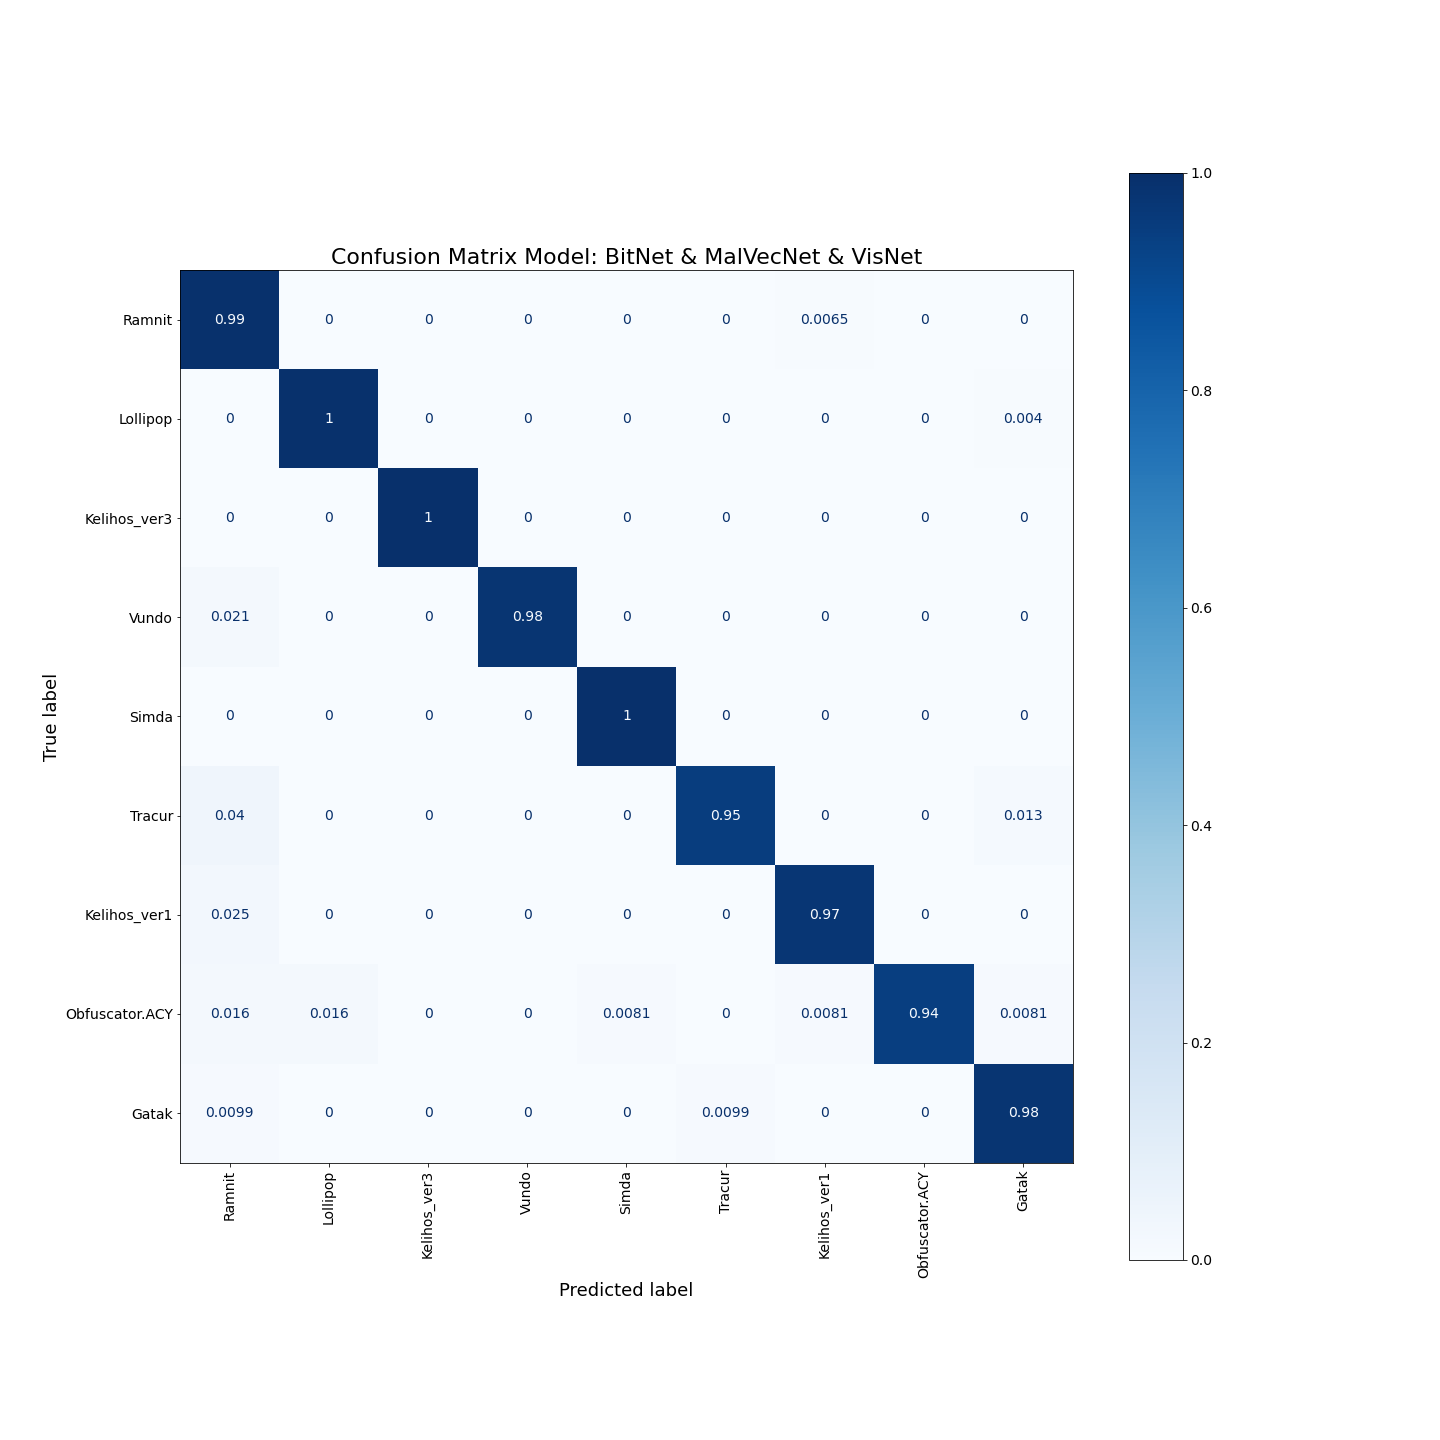
\includegraphics[scale=0.19]{img/confusion_matrix_2.png}
    \caption{EBANet confusion matrix without auxiliary output}
    \label{fig:a ensemble model confusion matrix without auxiliary output}
\end{figure} 


\subsection{Training Plots}
\counterwithin{figure}{subsection}
\setcounter{figure}{0}
\begin{figure}[H]
    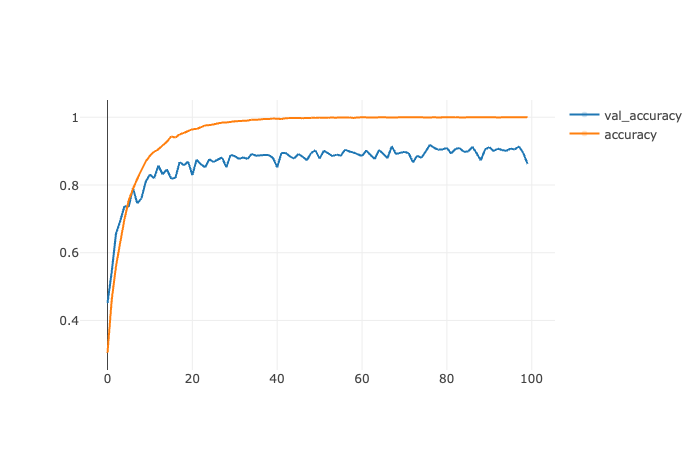
\includegraphics[scale=0.4]{img/malvecnet_training.png}
    \caption{ MalVecNet training plot}
    \label{fig:b MalVecNet training plot}
\end{figure}
\begin{figure}[H]
    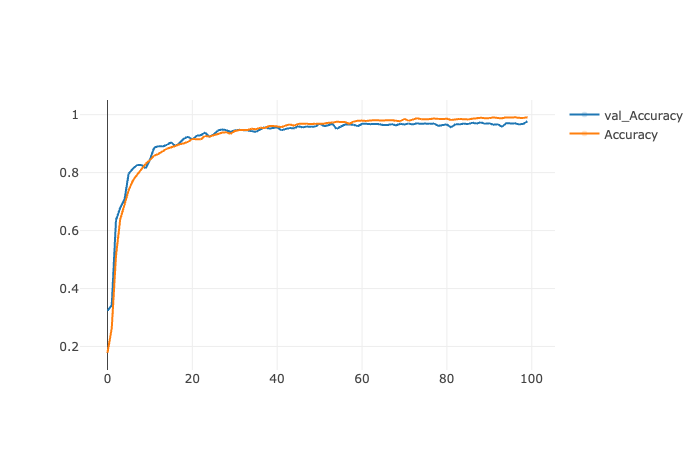
\includegraphics[scale=0.4]{img/bitnet_training.png}
    \caption{ BitNet training plot}
    \label{fig:b BitNet training plot}
\end{figure}    
\begin{figure}[H]
    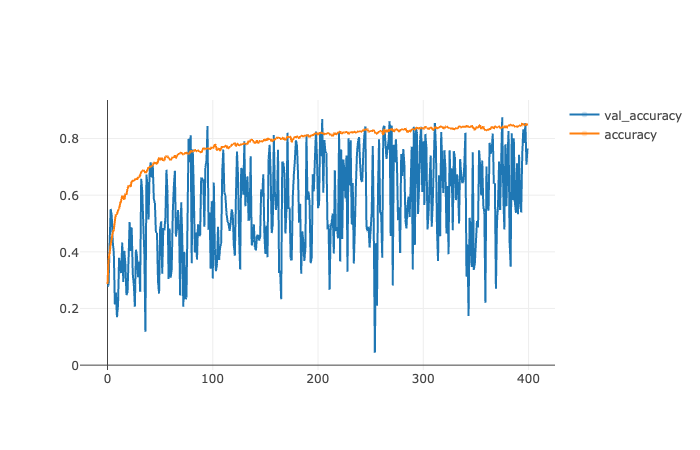
\includegraphics[scale=0.4]{img/visnet_training.png}
    \caption{ VisNet training plot}
    \label{fig:b VisNet training plot}
\end{figure} 
\begin{figure}[H]
    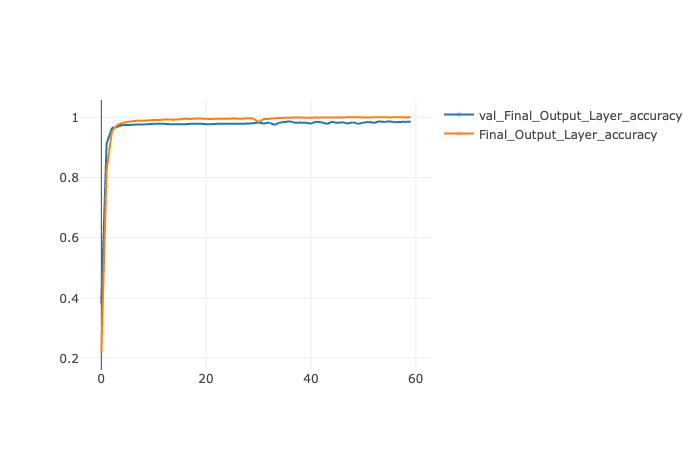
\includegraphics[scale=0.4]{img/ensemble_training_aux.png}
    \caption{ EBANet training plot with auxiliary outputs}
    \label{fig:b Ensemble training plot with auxiliary output}
\end{figure}       
\begin{figure}[H]
    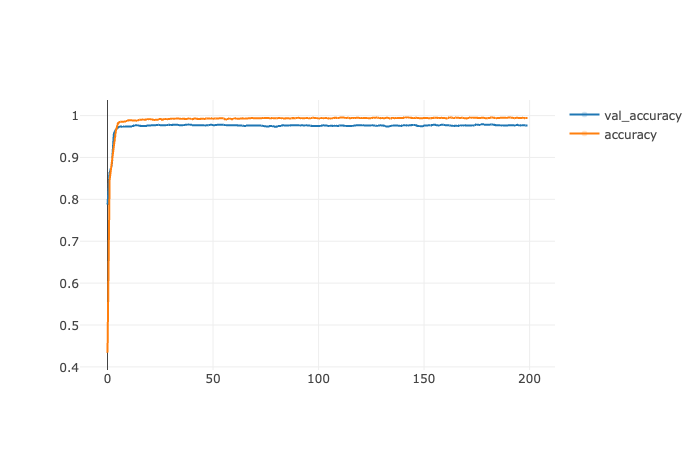
\includegraphics[scale=0.4]{img/ensemble_training.png}
    \caption{ EBANet training plot without auxiliary output}
    \label{fig:b Ensemble training plot without auxiliary output}
\end{figure}    

\end{document}
